\documentclass[a4paper, twosided, openany]{memoir}
\usepackage{hyperref}
\hypersetup{
	colorlinks,
	   linkcolor={black},
           citecolor={black},
           urlcolor={blue}
}
\usepackage{graphicx}

\setlrmarginsandblock{3cm}{2.5cm}{*}
\setulmarginsandblock{2.5cm}{2.5cm}{*}
\checkandfixthelayout
\setlength{\evensidemargin}{\oddsidemargin}

\begin{document}

\pagestyle{plain}
\chapterstyle{demo3}
\title{Advanced HTML XBlock for Open EdX platform}
\date{\today}

\frontmatter

%\maketitle

\chapter*{Certificate of Approval}

\begin{center}
\textsc{\LARGE Summer Internship 2018 Project}\\
\bigskip
\textsc{\Large Approval Certificate}\\
\bigskip
\textsc{ Department of Computer Science \& Engineering, IIT Bombay}\\
\textsc{--------------------------------------------------------------------------------------------------}\\
\bigskip\bigskip\bigskip\bigskip\bigskip\bigskip

The project entitled "Advanced HTML XBlock for Open EdX platform" submitted by Mr. Ashutosh Sathe, Mr. Srijan Roy Choudhury and Ms. Pravallika Podugu is approved for Summer Internship 2018 programme for 16th May 2018 to 6th July 2018, at Department of Computer Science and Engineering, IIT Bombay
\end{center}

\chapter*{Declaration}
\begin{center}

\end{center}

\chapter*{Abstract}
The project focuses on enhancing the open edx html component. Current html component does not
allow a fully fledged html, css and javascript content to be added in course. Also the html editor of
the current component is not very user friendly and lacks some fundamental functionalities such as
code indentation, code folding etc. Our first approaach was to modify openedx system itself and
thus changing the html editor for all users. Lateron we decided to move to devloping an xblock for
this and hence making it optional. We also added extra features to enahance the functionality of
xblock. These extra features include live previewing the html content along with editor.\newline
\par\fancybreak{$***$}\par

% Using newpage instead of pagebreak keeps the vertical alginment
% pagebreak will spread the content all over the page and that is why we had center alignment before
% This completely fixes it
\newpage

\chapter*{Acknowledgement}
	We, the summer interns of this group, are overwhelmed in all humbleness and
gratefulness to acknowledge our deep gratitude to all those who have helped us put
our ideas to perfection and have assigned tasks well above the level of simplicity and
into something concrete and unique.
We, wholeheartedly thank Prof. D.B. Phatak for having faith in us, selecting us to be
a part of his valuable project and for constantly motivating us to do better.
We thank Miss Kalpana Kannan for providing us the opportunity to work on this
project.We are also very thankful to our mentors Mr. Hitesh Murkute and Mr. Sachin R Shirsat
for their valuable suggestions. They were always there to show us the right track when needed help.
With help of their brilliant guidance and encouragement, we all were able to complete
our tasks properly and were up to the mark in all the tasks assigned. During the
process, we got a chance to see the stronger side of our technical and nontechnical
aspects and also strengthen our concepts.
Last but not the least, we wholeheartedly thank all our other colleagues working in
different projects under Prof. D.B Phatak for helping us evolve better with their critical advice.\newline
\par\fancybreak{$***$}\par
\newpage

\tableofcontents

\mainmatter

\chapter{Introduction}

Open edX is a widely used and very popular MOOC platform. The Open edX software is a opensource
technology that makes learning easier and studying faster. It was created by MIT and
Harvard University, and was quick to gain support of universities such as UC Berkely, Georgetown,
and Stanford.
The software platform is designed to engage students and teachers in an interactive, modular way. It
promotes active learning by video snippets, interactive components and game-like experience. The
course content is presented through learning sequences: a set of interwoven videos, readings,
discussions, wikis, collaborative and social media tools, exercises and materials with automatic
assessments and instant feedback.
The Open edX project is a global success. It powers major MOOC initiatives, hosting blended and
online courses, all around the world.
\chapter{Getting started}
\section{Limitations of the present HTML editor in OpenEdx}
Open edX in itself is a humongous learning management system with unparalleled feature list. It is
among the top MOOCs platforms in the world. As it is the way of the world, there is nothing perfect
here and Open edX is not an exception. All applications/platforms have a scope to enhance its
features and abilities of its components. In this project we worked on enhancing the HTML
component which is used for content creation in courses.\newline\newline
While current HTML editor does the job well but it has got its own mind and behaves with
uncertainty sometimes. Enhancing the editor with internal CSS and ironing out the indentation
issues will boost the user experience of the course creator. Our aim was to develop and integrate a
full-fledged HTML editor like Notepad++ or Sublime for Open edX.\newline\newline
Here are some issues that we have encountered in the HTML editor used by the OpenEdx platform
\begin{enumerate}
  \item \textbf{Indentaion in the current HTML editor :-}\newline\newline
The purpose of code indentation and style is to make the program more readable and
understandable. It saves lots of time while we revisit the code and use it.
Code indentaion in an important part towards increasing the aesthetic of any editor,
as it increases readability and makes understanding of the code easier.\newline\newline
In Open edX however the code indentation feature is not implemented in the raw
HTML editor, which is the CodeMirror v3.21.0. This is mainly because the version
of CodeMirror used in Open edX has been implemented with a minimalistic use case
and has not been updated since October 2015. The problem is that even if we
manually indent our code, once we save our progress and close the raw editor, the
indentation is lost i.e it doesn’t gets saved. 

  \item \textbf{Code Folding in the current HTML editor :-}\newline\newline
Code folding is a feature of some text editors, source code editors, and IDEs that
allows the user to selectively hide and display – "fold" – sections of a currently edited
file as a part of routine edit operations. This allows the user to manage large
amounts of text while viewing only those subsections of the text that are specifically
relevant at any given time.\newline\newline
This is a pretty useful feature for any editor and presents the user with various use
patterns, primarily organizing code or hiding less useful information so one can
focus on more important information. Since the CodeMirror version implemented in
Open edX is very old this feature is not available and thus was added to our List of
possible enhancements.

  \item \textbf{Internal CSS in HTML Code :-}\newline\newline
Cascading Style Sheets (CSS) is a style sheet language used for describing the
presentation of a document written in a markup language like HTML CSS is a
cornerstone technology of the World Wide Web alongside HTML and JavaScript.\newline\newline
The three main types of CSS styles are inline, internal and external. Currently in
Open edX platform in the raw HTML editor only inline or embedded CSS support is
available. Inline styles are CSS styles that are applied directly in the page's HTML.
Because inline styles they are the most specific in the cascade, they can over-ride
things we didn't intend them to. They also negate one of the most powerful aspects
of CSS - the ability to style lots and lots of web pages from one central CSS file to
make future updates and style changes much easier to manage.\newline\newline
If we had to only use inline styles, our documents would quickly become bloated and
very hard to maintain. This is because inline styles must be applied to every element
we want them on. That is why internal CSS is preferred whenever exhaustive use of
CSS is required as opposed to inline CSS. Internal CSS is Open edx raw HTML
editor is not supported as internal CSS must be defined inside the style tag in the
head element of the html body. However the raw HTML editor of Open edX stips
down style tags and the effects are not reflected as wanted. Styles of other
components in the web page also gets changed which we do not want. Thus allowing
internal CSS is an important enhancement criterion which should be addressed.
\end{enumerate}

To understand the limitations better we have provided the screenshots as mentioned
below:
\begin{center}\textbf{[See Figures 1-4 in the “Figures and Screenshots” section.]}\end{center}


\section{Objectives}
Here are the list of enhancements we were aiming for in the html component of Open edX:
\begin{itemize}
  \item Improvise the raw HTML editor to have features like pretty indentation, code folding
etc.
  \item Check if we can add a separate CSS section in raw HTML editor to eliminate inline
CSS
\item Fix the cursor placement issue and some other minor issues.
\end{itemize}

\section{Observations}
Regarding the Open edX paltform and the editors used in the Open Edx one might come up with thefollowing kind of questions
\begin{itemize}
\item Is OpenEdx using a raw editor or visual editor or both ?
\item Did OpenEdx write their own editor ?
\item If yes, then what how is it working ?
\item If no, then from where they have implemented their text editors
\item What kind of editor are they using ?
\item Where do we find the editors source code ?
\item How many editors are they using ?
\item Their method of working ?
\item Their current scenario ?
\item On what basis is this editor working along with the OpenEdx platform ?\newline\newline
\end{itemize}


To all these queries here are some facts that would be helpful:
\begin{enumerate}
\item OpenEdx uses both the visual editor as well as the raw editor.
\item OpenEdx has not written their own editor neither the visual editor nor the raw editor.
\item OpenEdx uses open source text editors for this purpose.
\item The visual editor is tinyMCE editor and the raw editor is CodeMirror Editor.
\item These editors are located in edx source code, in github.
\item CodeMirror is made to work in the custom mode configuration. OpenEdx is using a very old version of CodeMirror.
\item The tinymce editor folder of openedx consists of a plugin called "codemirror-for-tinymce".
\item The good thing about this plugin is that any version of codemirror can be used in the code and it will work perfectly fine.
\item The “codemirror-for-tinymce” plugin is already in use in the OpenEdx repository.
\item We can use the “codemirror-for-tinymce” plugin for tinymce 4.x.x versions.
\item There is an xblock module or simply an xblock called html-module.py
\item This particular xblock module handles the operation of the html editor.
\item This is the module that loads the html editor widget and configures both (tinymce and codemirror) editors to work hand in hand with the help of “codemirror” plugin for tinymce.
\end{enumerate}


\section{Our plan of action}

Depending on the facts that we uncovered regarding the html editors we have come up with
two possible approaches initially, that would fulfill our required objectives.
\begin{enumerate}

\item\textbf{Approach I}\newline Updating the present version of WYSIWYG and raw HTML editors in Open
edX
\item\textbf{Approach II}\newline Integrating other third party open source text editors into OpenEdx platform.
\end{enumerate}

%%%%%%%%%%%%%%%%%%%%%%%%%%%%%%%%%%%%%%%%%%%%%%%%%%%%%%%%%%%%%%%%%%%%%%%%%

\chapter{Approach I - Local integration}
\section{Updating the present version of Editors present in Open edX}
Our first approach was to download the latest versions of TinyMCE, CodeMirror and
the plugin “codemirror-for-tinymce” from their respective git repositories into our local
Machine.\newline
Next step was to integrate the two editors i.e., CodeMirror and TinyMCE using the plugin and
test it on our local machine, and later integrate it with Open edX using one of the Open edX developing
environment.\newline
The result would be TinyMCE loading the instance of latest version of CodeMirror as its
raw HTML editor.
However this implementation could only solve the indentation and code folding problem,
but still the internal css problem wouldn’t be solved just with this.\newline\newline
For enabling the internal CSS we thought of two possible implementations:
\begin{enumerate}
\item\textbf{Using Iframes}\newline
For this, we were planning to wrap the entire html content inside an iframe
and then add theming to the iframe.
\begin{itemize}
\item Set the width of iframe to 100\%
\item Set the height of iframe equal to the height of content of iframe
\item Set the border of iframe to zero/none
\item Open all hyperlinks within the iframe in new tab
\end{itemize}
Hence the expected result is an invisible iframe holding our HTML content.



\item\textbf{Using JavaScript}\newline
This is a slightly tough and critical approach, which was to apply CSS using
JavaScript. The plan was to separate out CSS part from HTML content and
wrap the entire content in a html div tag with an unique id.
Next we would have to manually select each and every child of the div by
parsing the DOM (Document Object Model) tree and apply styles to it.\newline
\end{enumerate}

We opted for the first i.e the Iframe approach because of the following reasons:
\begin{enumerate}
\item This method allows the course content creator to include third party CSS such as
bootstrap, w3css which will make the course even more beautiful
\item Implementaion is easier
\item Wrapping data inside the iframes containerizes the data ensuring no mixing of
CSS between two HTML blocks in LMS.
\item The overhead of the second approach will be very large, since parsing
the DOM tree would take considerable amount of time and effort.
\end{enumerate}


\section{Implementation of our Local integration}
In the first phase of implementing our approach of updating the present editors, we
first downloaded both the editors onto our local machine and then integrated the latest
version of CodeMirror and TinyMCE in our local machine. Later we integrated it with
Django framework since Open edX uses Django framework in the back end as their Web
Application Framework. This step was done to give us a better insight into the interaction of
the present editors in Open edX with Django. The steps of our implementation are
mentioned in brief below:
\begin{enumerate}
\item Firstly, we had downloaded the latest version of CodeMirror and TinyMCE from their
github repositores and then tested them individually to check whether all the desired features
are working or not.
\item Secondly, we had downloaded the latest version of the “codemirror-for-tinymce” plugin
from its git repo.
\item Next we had replaced the default raw HTML editor of TinyMCE with our instance of the
latest version of CodeMirror. This was done by configuring the \textbf{init-tinymce.js} file to use
CodeMirror as an external plugin and thus load it as its default raw HTML editor.
\item Later, for enabling the internal CSS we had encapsulated the entire html content of the
editor into an iframe.
\item We have then set the width of the iframe to 100 percent and set the height of the iframe
equal to the height of the html content.
\item  We had made sure that the borders of iframe was set to zero to make it invisible so that
the user experience is better and smooth.
\item After completing our stand alone integration we merged it with a Django project to run
our editor as an app in the Django server. This integration was quite useful as Open edX
itself uses Django framework in its backend and it helped us in understanding about the
Django back end of Open edX.
\end{enumerate}


\section{Summary of our local integration}
After completing our local integration, firstly we had tested our local instances of
TinyMCE and CodeMirror on the Django server. A brief summary of our observations are
listed below.
\begin{enumerate}
\item Most of the HTML tags and their atrributes are working fine. Some of the exceptions
being script tag , audio tag etc.
\item Almost every CSS style and attributes work fine. The exceptions are those style features
which by default require a script tag to be implemented.
\item CSS animations can be implemented and other third party HTML-and CSS-based design
templates such as Bootstrap can be linked and used without any error.
\item We prepared a detailed Test Report which can be found here:\newline[\url{https://docs.google.com/spreadsheets/d/1AJQWfAG2NIjpxFZt2fnLPlKdhP2-q35KZ0DOmdb-F0w/edit#gid=0}]
\item  Source code is available in our github repository here:\newline[\url{https://github.com/ashutoshbsathe/codemirror-in-tinymce}]
\end{enumerate}


\section{Issues faced and solutions}
\begin{enumerate}

\item\textbf{AJAX:}\newline\newline
We had no idea about how to pass data between RESTful APIs at first. Then later we
found out that this can be done via a request called as AJAX which basically passes
the data in JSON format from one API to another API. And hence we used the same.
On a button click in our html, we would send the AJAX query from webpage to
Django backend. While this seems easy at first, it is a bit tricky when we are using
only a single text area and not entire form element. So the main problem was our
csrf\_token was not being set correctly since we were not using a form. So we
decided to completely skip the csrf authentication by adding @csrf\_exempt
decorator to our view

\item\textbf{Stripping of style tags:}\newline\newline
So tinyMCE does not allow you to directly add CSS in your html. It will constantly
filter out your own \verb=<style>= and \verb=<link>= tags out of it’s display content. The only way
to get around this is by setting valid\_children, valid\_elements and
extended\_valid\_elements properly in TinyMCE config.

\item\textbf{Indentation in the “CodeMirror with TinyMCE setup” :}\newline\newline
Now because the tinymce keeps filtering out content, there’s no actual way to show a
nice indented code in CodeMirror. For this we found a script that will indent our
html code nicely and we called it before setting the content in CodeMirror. One thing
to note here is that whatever indentation that was done in CodeMirror was a bit of a
pseudo Indentation and not true indentation as the course creator wants. Sure, it was
nicely indented, but if somewhere content creator specifically wanted a specific tag
on multiple line such as
\begin{verbatim}
<a href=”https://www.google.com”>
A SearchEngine
</a>
\end{verbatim}
It won’t be rendered in that way because the script treats anchor tag as a single-line
tag and it will be rendered as follows:
\begin{verbatim}
<a href=”https://www.google.com”>ASearchEngine</a>
\end{verbatim}
Sadly enough, there is no way for tinyMCE to shut down it’s content filtering and
hence this issue remains unsolved.


\item\textbf{Unnecessary modification of html code:}\newline\newline
This issue specifically occurs when you try to edit something that was added in raw
mode. For example, let’s hope you add a nice CSS animation and then return back to
tinyMCE for saving the content, while returning back, you accidently clicked in the
div of your animation and you pressed enter. Then tinymce will try to split your div
in half breaking it where you pressed enter, and will also add some bad html code
which you definitely don’t want. Again this issue is unavoidable because of content
filtering algorithms used in tinyMCE.
\end{enumerate}

%%%%%%%%%%%%%%%%%%%%%%%%%%%%%%%%%%%%%%%%%%%%%%%5

\chapter{Research about Approach II}
\section{Integration Of The other third party Editors}
Just like CodeMirror and TinyMCE there are other third party open source text editors
which meet all the prerequisites of our enhancement critera. Some of them are Notepad++,
Quill, Brackets, ContentTools, Grapejs,etc. As an alternative to our first approach we
thought of another possibility of reaching our objective. Just like how the OpenEdx has
merged two text editors for their HTML editor, similarly even we can try to integrate
WYSWYG editor using the same methodology. In this approach we develop an entire new
editor itself. Moreover since all these editors are open source their github repositories is
easily accessible. So we also thought of trying to import the logic they used in their source
code to add features such as code indentation ,code folding etc. We put this approach as our
backup for our approach1 because, approach2 is a bit hacky and complicated to implement
compared to approach1. 
\section{What kind of editors do we want?}  
Before integrating here are some of the questions that we asked ourselves. \newline
\begin{itemize}
\item What kind of editor do we want...??
\item What features does that editor should have..??
\item How does these editors help with our motive..?? \newline 
\end{itemize}
So here are few points that helped us clear our doubts: \newline
\begin{itemize}
\item We need an editor that makes our work easy, simple, and has got much better working
properties as compared to the editor that is currently being used in the OpenEdx platform.
\item The editor should have inbuilt features(code folding, pretty indentation,languages,etc) that
could just wipe out the issues that are being faced by the openEdx html editor.
\item Since our motive is to add features such as indendation , cold folding, internal css,etc, so
considering an editor that has these features inbuilt, and integrating it by making some
required changes might help us in achieving our motive, and would even resolve in
eliminating the issues faced by the current HTML editor that is being used by the OpenEdx
platform. \newline
\end{itemize}

After a bit of research work what we found out is some pretty good and well built editors
that support html language. All these editors are open source and all their source code is
available in their respective git repositories. The list of editors that we had researched on
are as follows: \newline
\begin{itemize}
\item Notepad++
\item Brackets
\item ContentTools
\end{itemize}
The detailed explanation about each editor follows.
\section{Notepad++}
\subsection{About}
Notepad++ is a free (as in “free speech” and also as in “free beer”) open source code editor
and Notepad replacement that supports several languages. Running in the operating system
its use is governed by the GPL license. \newline\newline
As of now the current version of the Notepad++ available in the market is v7.5.6. \newline
\subsection{Features} 
\begin{enumerate}
\item Syntax Highlightning
\item Syntax Folding
\item User Desfined Syntax Highligting and Syntax Folding. (images (n++1,2,3,4))\item PCRE (Perl Compatible Regular Expreession) Search and Replace.
\item GUI entirely customizable.
\item Auto completion: Word completion, Function completion and Function parameter hint.
\item Multi document (Tab interface).
\item Multi view
\item WYSIWYG (printing).
\item Zoom in and Zoom out.
\item Multi language environment supported.
\item Macro recording and playback.
\item Bookmark.  \newline
\end{enumerate}
\subsection{Observations Made} 
Here are a list of things that we have found about notepad++ : 
\begin{itemize}
\item Scintilla is the main component of Notepad++ which is very powerful.
\item This editor is written in c++
\item All the syntax styling part is done using the Scintilla component.
\item Scintilla edits and even is used for debugging the source code of the Notepad++
\item Some files where the required changes are to be made and importing those files so they can
be used in building an editor for OpenEdx platform. \newline
\end{itemize}  

\subsection{Idea Of Implementation }
In a similar way in which the Open edX platform uses an xmodule(html\_module.py) that
handles the operation of its current html editor, similarly, using the same working principle
we can replace our editor and load the html editor and configure it for proper working.  
\section{Adobe Brackets}
\subsection{About}
With focused visual tools and preprocessor support, Brackets is a modern text editor that
makes it easy to design in the browser. It's crafted from the ground up for web designers and
front-end developers. \newline 
Brackets is an open source editor written in HTML, CSS, and JavaScript with a primary
focus on web development. It was created by Adobe Systems, licensed under the MIT
License, and is currently maintained on GitHub by Adobe and other open-sourced
developers. Brackets is available for cross-platform download on Mac, Windows, and is
compatible with most linux distros. The main purpose of brackets is its live html, css and js
editing functionality.
\subsection{Features}
\begin{enumerate}
\item Quick Edit
\item Quick Docs
\item Live element debugging
\item Live preview
\item Inline Editors
\item Split View
\item Thesus Integration
\item LESS support
\item W3C Validation
\item Drag and Drop
\item Auto Prefixer
\item Git Integration for Brackets
\item JS Lint
\end{enumerate}
\subsection{Observations Made}
Here are a list of things that we have found out about Brackets: \newline
\begin{itemize}
\item Brackets is written in JavaScript
\item Its an automated WYSIWYG editor
\item Mainly designed for web developers and front end developers
\item Applies quick edit for HTML elements which helps in displaying corresponding CSS
properties for that particular element.
\item When a color is typed it shows an inline color picker for our better convienience in
searching.
\item While writing the code it enables live preview , that works only for Google Chrome, and if
there is any html syntaxtical error then it forbiddens opening of the live prview.
\item Using this Thesus integration feature that enables inspecting an element in the real time and
debug any extension in brackets.
\item This uses CodeMirror text raw html editor for Code Formatting.
\item Brackets has got more than 20 Dependencies .
\item It consists of a bracket (which is a root module) that pulls in other modules as dependencies.
\item Some files where the required changes are to be made and importing those files so they can
be used in building an editor for OpenEdx platform
\end{itemize}
\subsection{Idea Of Implementation}
In a similar way in which the Open edX platform uses an xmodule(html\_module.py) that
handles the operation of its current html editor, similarly, using the same working principle
we can replace our editor and load the html editor and configure it for proper working.

\section{ContentTools}
\subsection{About}
ContentTools is a JavaScript/CoffeeScript library aimed at building WYSIWYG editors for
HTML content. ContentTools aims to provide both a fully-functional editor that can be used
out of box and a toolkit of classes, a set of tools for performing common editing tasks, and a
history stack for managing undo/redo. Whilst the components provided by the toolkit work
well together, they can also be used or replaced as required. \newline
\subsection{Features}
\begin{enumerate}
\item Easily integrated with any HTML document.
\item Drag and Drop directly within the page.
\item Floating context-sensitive toolbar.
\item Compatible with all major web browsers and operating systems.
\item The javaScript library can transform any HTML page into an WYSIWYG editor.
\item Countless possibilities for building wondrous interactive apps and services.
\item Media Resizing.
\end{enumerate}
\subsection{Observations Made}
\begin{itemize}
\item Allows text content, images, embedded videos, tables and other page content to be
edited, resized, or moved using the Drag and Drop property within the page itself.
\item Requires bower or npm for installation.
\item For building library’s and project, requires grunt node modules and SASS.
\item Uses an HTML string for formatting rather than using an HTML parser written in
JavaScript.
\item Its library uses a minimal finite state machine(FSM) for JavaScript.
\item It consists of an JS library that provides cross-browser support for content selection.
\item It has a javascript library that provides a set of classes for building content editable
HTML elements.
\item The ContentTools editor has already been implemented into the content management
systems of a number of websites.
\item This editor is a recent editor which has got wonderful, simplified and an unique
UserInterface.
\item Its Framework integration includes “Django REST Framework” and “Image
Uploads with Cloudinary”.
\item ContentTools is part of a collection of JavaScript libraries (ContentTools,
ContentEdit, ContentSelect, FSM, HTMLParser) which were developed to aid in the
creation of HTML WYSIWYG editors.
\item It has an ability to configure styles for your content.
\item Contenttools can be easily integrated into the CMS.
\item It is an opensource web-based HTML editor whose working is quite similar to
CodeMirror and TinyMCE, so integrating with the OpenEdx platform would be
quite simpler as all of then belong to the same working methodology.
\end{itemize}
\subsection{Idea Of Implementation}
In a similar way in which the Open edX platform uses an xmodule(html\_module.py) that
handles the operation of its current html editor, similarly, using the same working principle
we can replace our editor and load the html editor and configure it for proper working.  \newline
\newline
Integrating this would be much easier compared to Brackets and Notepad++ as its working
methodology is just as similar to the CodeMirror and TinyMCE which are being used as of
now in the OpenEdx platform. \newline
\subsection{Installation Issues}
Installing Notepad++ and Brackets easy was error free but with ContentTools the only issue
that occurred while installing was related to the npm package installer. \newline
The packages were not completely installed and hence npm threw an error while
installing. \newline \newline
Here is the log file that shows the errors that would be occurring , \newline 
[\url{https://drive.google.com/open?id=1KUe3jcAPg8DpxmhshPUBYPKya_B-oRSt}]
\newline 
\newline
\textbf{SOLUTION :} To resolve this issue here are the things that are to be followed: \newline
\begin{enumerate}
\item Open your terminal and perform the following operations 
\begin{center}\verb=sudo apt-get update synaptic=\end{center}
\item A dailog box opensSearch for npm and node modules
\item Delete those folders manually
\item Save the changes and close the dialog.
\item Open the terminal and type in the following commands
 \begin{center}\verb=npm install --save ContentTools=\end{center}

\end{enumerate}
\section{Advantages Of Approach1 Compared To Approach2}
\begin{enumerate}
\item Upgrading something is always better than integrating something new altogether. As per
our research and observation the versions of CodeMirror and TinyMCE in Open edX are
outdated. Since the latest versions of these two editors fullfill our requirements updating the
editors is much straighforward and sensible than incorporating two completedly new ediitors
into the Open edX platform, since it can lead to a lot of dependency issues.
\item The iframe approach also allows the course content creator to include third party CSS
such as bootstrap, w3css which will make the course even more interactive and boost
student experience. Course creators can style their courses with a variety of such third party
CSS features and make it a lot more interactive for the students.
\item Wrapping data inside the iframes containerizes the data ensuring no mixing of CSS
between two HTML blocks in LMS. This is very important in order to provide an error free
user experience.
\end{enumerate}


\section{References}
The following links would be helpful in learning more about the working of the editors discussed previoulsy
\begin{enumerate}
\item\textbf{Notepad++}
\begin{itemize}
\item \url{https://github.com/notepad-plus-plus/notepad-plus-plus}
\item \url{https://github.com/notepad-plus-plus/notepad-plus-plus/blob/master/scintilla/lexlib/Accessor.cxx}
\item \url{https://github.com/notepad-plus-plus/notepad-plus-plus/blob/master/scintilla/src/AutoComplete.cxx}
\item \url{https://github.com/notepad-plus-plus/notepad-plus-plus/tree/master/scintilla/lexers}
\item \url{https://github.com/notepad-plus-plus/notepad-plus-plus/tree/master/scintilla/lexlib}
\end{itemize}
\item\textbf{Adobe Brackets}
\begin{itemize}
\item \url{https://github.com/adobe/brackets}
\item \url{https://github.com/adobe/brackets/blob/master/src/styles/brackets_codemirror_override.less}
\item \url{https://github.com/adobe/brackets/tree/master/src/LiveDevelopment}
\item \url{https://github.com/adobe/brackets/blob/master/src/LiveDevelopment/Agents/CSSAgent.js}
\item \url{https://github.com/adobe/brackets/blob/master/src/editor/}
\item \url{https://github.com/adobe/brackets/tree/master/src/htmlContent}
\end{itemize}
\item\textbf{ContentTools}
\begin{itemize}
\item \url{https://github.com/GetmeUK/ContentTools}
\item \url{https://github.com/Cotidia/django-contenttools-demo}
\item \url{http://getcontenttools.com/api/content-select}
\item \url{http://getcontenttools.com/tutorials/content-tools-plus-cms}
\end{itemize}
\end{enumerate}



\chapter{Setting up a development environment for Open edX platform}

\section{Open edX installation options}
In order to test our local integation what we needed was a running instance of Open edX platform
on our local machine. Open edX has provided us with different installation options depending on
our use. They are described in brief below.
\begin{itemize}
	\item \textbf{Devstack:} useful if we want to modify the Open edX code. The code will be in directories
shared between the host and the guest operating systems. We should run the code in the
guest, but can edit it in the host, where we can use our own tools.
		\begin{enumerate}
		\item For Ginkgo and earlier, devstack was a Vagrant installation.
		\item For Hawthorn, devstack is based on Docker. An unsupported pre-release is
available.
		\end{enumerate}
	\item If we want to run a production installation and want a production like environemnt on our
local machne then we can use \textbf{Native} or \textbf{Manual} installation. The Native installation installs
the Open edX software on our own Ubuntu 16.04 machine in a production-like
configuration.
	\item If we want a production-like installation for testing, we can use \textbf{Fullstack} or \textbf{Native}.
Fullstack is a Vagrant instance designed for installing all Open edX services on a single
server in a production-like configuration. Fullstack is a pre-packaged Native installation
running in a Vagrant virtual machine.
\end{itemize}
Since our project deals with making changes in Open edX source code we naturally opted for Devstack, which is designed for developers

\section{Open edX Devstack}
Devstack is traditionally a Vagrant instance designed for local development. Devstack has the same system
requirements as Fullstack. This allows us to discover and fix system configuration issues early in
development. Devstack simplifies certain production settings to make development more
convenient. For example, nginx and gunicron are disabled in devstack; devstack uses Django’s
runserver instead in conformation with Open edX platform.\newline
Devstack is maintained as a set of docker containers lately and hence we chose that way as well

\section{Installing a docker based devstack}

\subsection{Prerequisites}
\begin{itemize}
	\item This installation requires Docker 17.06+ CE. It is recommended to use docker stable, but docker edge should work as well
	\item GNU-Make
	\item pip
\end{itemize}
\textbf{Note : }\newline
Linux users should not be using the \verb|overlay| storage driver. \verb|overlay2| is tested and supported, but requires kernel version 4.0+. We can check which storage driver our \verb|docker-daemon| is configured to use through following command : \newline
\begin{center}{\verb=docker info | grep -i 'storage driver'=}\end{center}

\section{Installing docker and docker compose}
Please note that, docker based devstack needs a fairly powerful computer. Our computer was using quad core core i5 7500u CPU with 8 GB RAM. Also, give more space to \verb=/= partition because docker needs more space for storing images.If you already have configured docker on your distro, you can skip this section. For following this guide, we recommend using any debian based distro where you would be able to use \verb=apt= package manager. 

\subsection{Getting docker for ubuntu}
Before we install Docker CE for the first time on a new host machine, we need to set up the Docker
repository. Afterward, we can install and update Docker from the repository. The steps are
mentioned below :
\begin{itemize}
	\item Update the \verb=apt= package index: \newline \begin{center}{\verb=$ sudo apt-get update=}\end{center}
	\item Install the packages to allow \verb=apt= to use a repository over \textbf{HTTPS}
		\newline \begin{center}{\verb=$ sudo apt-get install apt-transport-https \ =}\end{center}
		\begin{center}{\verb=ca-certificates curl software-properties-common=}\end{center}
	\item Add docker's official GPG key : \newline
		\begin{center}
		\verb=curl -fsSL https://download.docker.com/linux/ubuntu/gpg | sudo apt-key add -=
		\end{center}
		Verify that you now have the key with the fingerprint \verb=9DC8 5822 9FC7 DD38= \newline \verb=854A E2D8 8D81 803C 0EBF CD88= by searching the last 8 characters of the fingerprint\newline\newline
		\verb=$ sudo apt-key fingerprint 0EBFCD88=
		\begin{center}
			\begin{verbatim}
>> pub 4096R/0EBFCD88 2017-02-22
Key fingerprint = 9DC8 5822 9FC7 DD38 854A E2D8 8D81 803C 0EBF CD88
uid Docker Release (CE deb) <docker@docker.com>
sub 4096R/F273FCD8 2017-02-22
			\end{verbatim}
		\end{center}
	\item Use the following command to set up the \textbf{stable} repository. You always need the \textbf{stable}
repository, even if you want to install builds from the \textbf{edge} or \textbf{test} repositories as well. To
add the edge or test repository, add the word \textbf{edge} or \textbf{test} (or both) after the word 
\verb=stable= in the commands below.
		\begin{verbatim}
$ sudo add-apt-repository \
"deb [arch=amd64] https://download.docker.com/linux/ubuntu \
$(lsb_release -cs) \ stable"
		\end{verbatim}
\end{itemize}

\subsection{Installing Docker CE}
\begin{enumerate}
	\item  Update the \verb=apt= package index: \newline \begin{center}{\verb=$ sudo apt-get update=}\end{center}
	\item Install the latest version of Docker CE \newline \begin{center}{\verb=$ sudo apt-get install docker-ce=}\end{center}
	\item Docker should now be installed, the daemon started, and the process enabled to start on boot. To check that its running, we can use the following command\newline\begin{center}{\verb=$ sudo systemctl status docker=}\end{center}
\end{enumerate}

\subsection{Post installation steps for ubuntu}
\begin{enumerate}
	\item
	\textbf{Manage docker as a non root user}\newline
The docker daemon binds to a Unix socket instead of a TCP port. By default that Unix socket is
owned by the user root and other users can only access it using sudo. The docker daemon always
runs as the root user.
If we don’t want to use sudo when you use the docker command, create a Unix group called docker
and add users to it. When the docker daemon starts, it makes the ownership of the Unix socket
read/writable by the docker group.
To create the docker group and add our user:
	\begin{enumerate}
		\item Create the docker group \newline\begin{center}\verb=$ sudo groupadd docker=\end{center}
		\item Add our user to the docker group \newline\begin{center}\verb=$ sudo usermod -aG docker $USER=\end{center}
		\item Log out and log back in so that the group membership is re-evaluated. If testing on a virtual
machine, it may be necessary to restart the virtual machine for changes to take effect.\newline
On a desktop Linux environment such as X Windows, we need to log out of our session
completely and then log back in.
		\item Verify that you can run docker commands without sudo.\newline\begin{center}\verb=$ docker run hello-world=\end{center}
			This command downloads a test image and runs it in a coontainer. When the container runs, it prints an informational message and exits.
	\end{enumerate}

	\item
	\textbf{Configure Docker to start on boot}\newline
Most current Linux distributions (RHEL, CentOS, Fedora, Ubuntu 16.04 and higher) use \verb=systemd=
to manage which services start when the system boots. Ubuntu 14.10 and below use \verb=upstart=.
	\begin{enumerate}
	\item \verb=systemd= \newline\begin{center}\verb=$ sudo systemctl enable docker=\end{center}
		To disable this behavior, use \verb=disable= instead\newline
		\begin{center}\verb=$ sudo systemctl disable docker=\end{center}
	\item \verb=upstart= \newline
		Docker is automatically configured to start on boot using \verb=upstart=. 
		To disable this behavior, use the following command \newline
		\begin{center}\verb=$ echo manual | sudo tee /etc/init/docker/override=\end{center}
	\end{enumerate}
	\verb=chkconfig=
	\begin{center}\verb=$ sudo chkconfig docker on=\end{center}
\end{enumerate}

\subsection{Getting Docker compose for ubuntu}
On \textbf{Linux}, you can download the Docker Compose binary from the Compose repository page on git
hub. These step by step instructions are also included below.
\begin{enumerate}
	\item Run this command to download latest version of docker compose:
		\begin{center}
		\begin{verbatim}
		sudo curl -L
https://github.com/docker/compose/releases/download/1.21.2/docker-compose-
$(uname -s)-$(uname -m) -o /usr/local/bin/docker-compose
		\end{verbatim}
		\end{center}
		We should use the lates compose release number in download command. The above command is an example and it may become out-of-date. To ensure you have the latest version, check the compose repository on release page on GitHub \url{https://github.com/docker/compose/releases}
		\newline If you have problems installing with \verb=curl=, you can find alternative options in docker documentation.
	\item Apply the executable permissions to the binary\newline\begin{center}\verb=$ sudo chmod +x /usr/local/bin/docker-compose=\end{center}
	\item Test the installation
		\begin{center}
		\begin{verbatim}
$ docker-compose –version
>>docker-compose version 1.21.2, build 1719ceb
		\end{verbatim}
		\end{center}
\end{enumerate}

\section{Installing docker based devstack}
\begin{enumerate}
	\item Clone the git repository of devstack\newline
	\begin{center}
	\begin{verbatim}$ git clone https://github.com/edx/devstack && cd devstack
	\end{verbatim}
	\end{center}
	\item Install the requirements inside of a python virtualenv \newline
	\begin{center}
	\begin{verbatim}$ make requirements
	\end{verbatim}
	\end{center}
	\item The Docker Compose file mounts a host volume for each service's executing code. The
host directory defaults to be a sibling of this directory. For example, if this repo is
cloned to \verb=~/workspace/devstack=, host volumes will be expected in \verb=~/workspace/coursediscovery=,
\verb=~/workspace/ecommerce=, etc. These repos can be cloned with the command
below.\newline
\begin{center}
\begin{verbatim}make dev.clone
\end{verbatim}
\end{center}
We may customize where the local repositories are found by setting the
\verb=DEVSTACK_WORKSPACE= environment variable
	\item We must Run the provision command, if we haven't already, to configure the various
services with superusers (for development without the auth service) and tenants (for multitenancy).
When running the provision command, databases for ecommerce and edxapp will
be dropped and recreated.
The username and password for the superusers are both edx. We can access the services
directly via Django admin at the \verb=/admin/= path, or login via single sign-on at \verb=/login/=.\newline
\begin{center}
Default: \verb=make dev.provision=
\end{center}
	\item Start the services. This command will mount the repositories under the
\verb=DEVSTACK_WORKSPACE= directory. It may take up to 60 seconds for the LMS to start,
even after the \verb=make dev.up= command outputs done.\newline
\begin{center}
Default: \verb=make dev.up=
\end{center}
\end{enumerate}

Please note that all the above commands are to be executed in \verb=devstack= directory and \verb=DEVSTACK_WORKSPACE= MUST be exported correctly throughout the process.

After the services have started, if we need shell access to one of the services, we can run \begin{verbatim}make <service>-shell\end{verbatim}. For example to access the Catalog/Course Discovery Service, we can run:\newline
\begin{center}
\verb=make discovery-shell=
\end{center}
To see logs from containers running in detached mode, we can either use "Kitematic" (available
from the "Docker for Mac" menu), or by running the following:\newline
\begin{center}
\verb=make logs=
\end{center}
The screenshots of the running instance of our Devstack along with the LMS and CMS
section are provided as mentioned below:
\begin{center}
\textbf{[See Figures 5-8 in the “Figures and Screenshots” section.]}
\end{center}

\subsection{Service URLs}
Each service is accessible at \verb=localhost= on a specific port. The table below provides links
to the homepage of each service. Since some services are not meant to be user-facing, the
"homepage" may be the API root
\begin{center}
	\begin{tabular}{ |c|c| }
	\hline
	\textbf{Service} & \textbf{URLs} \\
	\hline
	Credentials & http://localhost:18150/api/v2/ \\
	Catalog/Discovery & http://localhost:18381/api-docs/ \\
	E-commerce/Otto & http://localhost:18130/dashboard/ \\
	LMS & http://localhost:18000/ \\
	Notes/edx-notes-api & http://localhost:18150/api/v1/ \\
	Studio/CMS & http://localhost:18010 \\
	\hline
	\end{tabular}
\end{center}
\section{Issues and solutions}
During the course of our Docker based installation and configuration of Open edX Devstack,
we faced multiple issues such as proxy settings etc. The issues are mentioned below along
with the solutions we used to overcome them.
\begin{enumerate}
	\item \textbf{Proxy configuration of the system :}\newline
		\begin{itemize}
		\item Initially we tried installing our instance of Open edX Devstack behind a proxy server. But
many packages mainly the ones which were being installed using pip were failing.
		\item We thought of trying to enable proxy inside the docker container, but due to the large
amount of time it took to resolve several layers of proxy authentication the reuqest was
getting timed out.
		\item Thus, the docker container was unable to fetch the required packages from Open edX.
		\end{itemize}
		\textbf{Solution :}After trying several times, we decided to discard the installation using a proxy.
We used normal mobile data to install all the require services and get our Devstack up and
running. With the help of mobile data the installation was completed error free and all the
packages were downloaded correctly.
	\item \textbf{Issue with docker installation : }\newline
		Docker isntallation can create some problems if the steps are not followed correctly and in
order. After installing Docker it is important to perform the post installation steps ,
because it happens sometimes that the system is unable to connect to the docker daemon.
	\item \textbf{Issues compiling static assets : }\newline
This is a package related issue. This can happen with any of the service randomly. The issue here is
the script that is building static assets for a particular service, needs only a specific version of npm
package “babel-loader”. Sometimes durirng the provisioning, it updates the package “babel-loader”
via npm. We could not exactly find out when the update was happening, it was random most of the
times. If you ever encounter issue with newer “babel-loader”, just modify the webpack to explicitly
tell the “babel-loader” to build JSX as ReactNative assets. Also it might give error about Object
Spread, all you need to do it to add plugin into your webpack\newline
The modified webpack can be found on our git\newline
Also check out :\newline

\begin{small}\url {https://stackoverflow.com/questions/33460420/babel-loader-jsx-syntaxerror-unexpected-token}\end{small} \& \newline
\begin{small}\url{https://babeljs.io/docs/en/babel-plugin-transform-object-rest-spread}\end{small}
	\item \textbf{Docker environment issues :} \newline
	\begin{figure}
		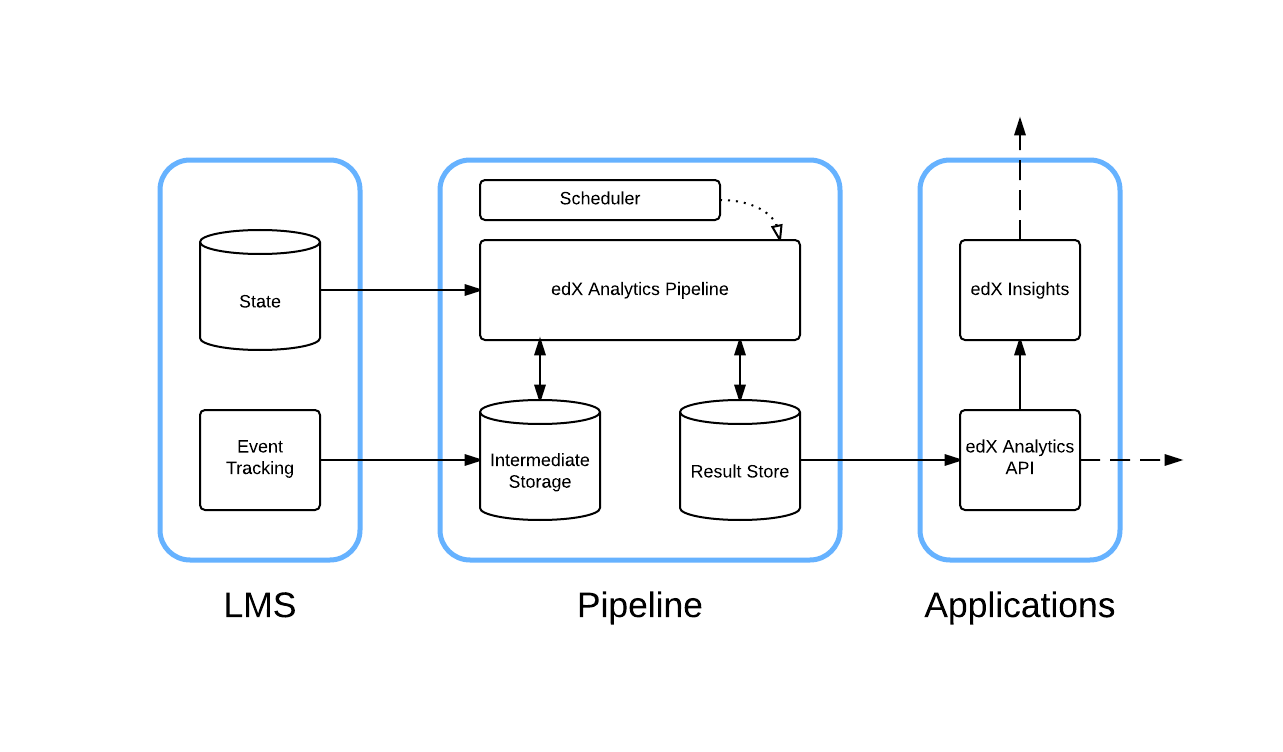
\includegraphics[width=\linewidth]{images/devstack_arch.png}
		\caption{Block diagram of devstack service}
	\end{figure}
As we can see in the diagram, every devstack service is made up of docker image and docker
volume. Docker images are pulled from openedx repos whereas volumes are mounted on your host
device. While mounting these docker volumes, script uses an environment variable called 
\verb=DEVSTACK_WORKSPACE= as shown in figure. It is highly probable that you set this variable
once and when retrying we forget to set this variable again. If we donot set this variable correctly
the mount silently fails and mounts a new volume instead. This is why it is necessary to set this
variable everytime you login into your host machine. For doing so, add the 
	\begin{center}
	\begin{verbatim}"export DEVSTACK_WORKSPACE=/path/to/your/workspace"
	\end{verbatim}
	\end{center} line at the bottom of your \verb=.bashrc.=
After doing “\verb=source .bashrc=” will export the variable correctly. To see whether the variable is set
correctly or not, type “\verb=printenv=”\newline
Important note for “\verb=sudo=”. If you are doing any command with sudo, make sure to preserve the
current environment variables. For doing so, use \verb=-E= flag with sudo to preserve them.
\end{enumerate}

%%%%%%%%%%%%%%%%%%%%%%%%%%%%%%%%%%%%%%%%%%%%%%%%%%%5555555

\chapter{Approach I- Open edX intregation}
After testing our hybrid local intregation, and setting up our developing environment for Open edX,
the next phase was to integrate it with the running instance of Open edX on our Devstack
\section{Plan of action}
The idea and plan behind intregating our running hybrid instance of CodeMirror in TinyMCE with
Open edX is mentioned below:
\begin{enumerate}
\item\textbf{Indentation and code folding features}
\begin{itemize}
\item Add the latest version of CodeMirror v5.38.0 to the source code of Open edX
leaving the older version untouched.
\item Configure TinyMCE to open the updated version of CodeMirror as its raw HTML
editor.
\item Test the updated CodeMirror in TinyMCE and see if its wroking as expected.
\end{itemize}
\item\textbf{Enabling internal CSS}
\begin{itemize}
\item Understand the working of the XModule html\_module.py which is the widget
which loads the WYSIWYG editor in Open edX.
\item Learn how the html content is getting stored in the MongoDB .
\item The idea was to wrap the html content inside an inframe before it gets stored in the
Database. However this was to be done only when the course authors used internal
CSS in thier courses.
\item Similarly, while loading the content in LMS, it would be wrapped inside and iframe
first and then rendered in order to produce the desired effect.
\end{itemize}
\end{enumerate}

\section{Implementation}
\subsection{Configuring TinyMCE to use updated CodeMirror v5.38.0}
\begin{itemize}
\item The CodeMirror and TinyMCE source files are located in the edx-platfrom can be found on
the following path : \textit{\textbf{edx-platform/common/statis/js/vendor}}
\item Inside the tinymce source code, we placed the updated version of CodeMirror in the plugins
folder for TinyMCE.\newline The path was :
\textit{\textbf{edx-platform/common/static/js/vendor/tinymce/js/tinymce/plugins}}
\item Next we configured TinyMCE to use the updated CodeMirror as its raw HTML editor. This
was done through making changes in the TinyMCE configuration file \textbf{edit.js} located here :\newline
\textbf{\textit{edx-platform/common/lib/xmodule/xmodule/js/src/html/edit.js}}
\item Similarly, while loading the content in LMS, it would be wrapped inside and iframe
first and then rendered in order to produce the desired effect.
\end{itemize}
After performing the following steps we were able to configure TinyMCE to open our updated
instance of CodeMirror v5.38.0 as its raw HTML editor succesfully. Features such as indentation,
code-folding etc were working fine

\subsection{Using Iframes to enable internal CSS}
\subsubsection{Issues faced}
Once we were able to intreagte updated version of CodeMirror with TinyMCE, we tried testing
internal CSS in our new editor. Our observations are mentioned below:
\begin{itemize}
\item  The effect of the internal CSS is only visible inside the WYSIWYG editor i.e inside
TinyMCE.
\item  Once we save our progress the Open edX backend automatically strips the style tag and
removes it. As a result of this, no effect of the CSS is visible in the actual course content.
\end{itemize}

\section{Change in Approach}
\subsection{What happened to the issues}
We tried to look into the issues by looking into openedx backend by logging at several places in
several different xmodules and we failed. We discussed this issue with Aparna Ma’am(Mentor,
IITBombayX team). She said that we were on a right track and we should play with backend
through logs itself. Strangely enough, there were NO logs generated at all!! This lead us to a
roadblock situation where we need to switch to another approach for checking out backend.
However, all of the ways went at least once through logging step which was not working on our
devstack very well. We also discovered that the server provided to us for R\&D
purposes(10.129.27.44) also was unable to generate any logs.
\subsection{Need for change in approach}
Because of these issues, we were facing a major roadblock ahead of us and hence we need to
switch approaches. Now we had 2 more options, Xblock and integrating entirely a new editor into
an already complex openedx system which does not even generate logs ! Another option was to
reinstall devstack and see what causes devstack to not generate logs. But the clock was ticking and
we only hand 2.5 weeks left for the internship period. We could have pursued approach 1 to the end
and maybe end the internship without completing the project but we chose to change approach.
\subsection{Why Xblock approach and not integrating editors such as
contenttools/grapejs ?}
Two main reasons:
\begin{enumerate}
\item If we wanted to integrate any of these with OpenEdx, we would need the logger to be working
perfectly. And as described in the issues above, that is what kept us from pursuing approach 1 itself
\item Xblocks are modular. If we decide to modify the system, we’re forcing the editor changes to all
users. And probably some of these users don’t even need this advanced editor and features. On the
other hand, if we make this into an xblock, it will be used by people who actually need it and know
how to use it. Also one hidden advantage of xblock is that they are largely platform independent.
Most of the xblocks do not need to be updated on every single version of openedx since the core
Xblock API remains unchanged.
\end{enumerate}
%%%%%%%%%%%%%%%%%%%%%%%%%%%%%%%%%%%%%%%%%%%%%%%%%


\chapter{Basics of developing an XBlock}
\section{Introduction}
XBlock is a way to create rich engaging courses. XBlock is a component architecture of edX, and a
course can be build from the different Blocks as pieces. On the other hand, XBlock will offer
APIs and structure for other modules in the edX to comunicate with the course content since all
other web applications in a online ecosystem needs to access the course content.\newline
XBlock is the software development kit for edX-MOOC and it is written in python2. XBlock
generally contains few python classes which create a small web application. So, to create new
xblocks, a new module called xblock-sdk has been open sourced. Creating a new xblock means
creating a simple python installable python package with a class derived from the XBlock.

\section{XBlock API and Runtimes}
Any web application can be an XBlock runtime by implementing the XBlock API. The
XBlock API is not a RESTful API. XBlock runtimes can compose web pages out of XBlocks that
were developed by programmers who do not need to know anything about the other components
that a web page might be using or displaying.

\section{XBlocks for Developers}
Developers can select from functionality developed by the Open edX community by installing an
XBlock on their instance of Open edX. Developers can integrate new or propriety functionality for
use in XBlock runtimes by developing a new XBlock using the supported XBlock API.\newline\newline
XBlocks are like miniature web applications: they maintain state in a storage layer, render
themselves through views, and process user actions through handlers. XBlocks differ from web
applications in that they render only a small piece of a complete web page. Like HTML \verb=<div>= tags,
XBlocks can represent components as small as a paragraph of text, a video, or a multiple choice
input field, or as large as a section, a chapter, or an entire course.
\section{Criteria}
One must design a XBlock to meet two criteria:-
\begin{itemize}
\item The XBlock must be independent of other XBlocks. Course teams must be able to use the
XBlock without using other Xblocks.
\item The XBlock must work together with other XBlocks. Course teams must be able to combine
different XBlocks in flexible ways.
\end{itemize}

\section{Building an Xblock}
\subsection{Instalingl XBlock Prerequisites}
To build an XBlock, we must have the following tools on our computer.
\begin{itemize}
\item Python 2.7
\item Git
\item A Virtual Environment
\end{itemize}
\subsubsection{Python 2.7}
To run the a virtual environment and the XBlock SDK, and to build an XBlock, we must
have Python 2.7 installed on our computer.
\subsubsection{Git}
EdX repositories, including XBlock and the XBlock SDK, are stored on GitHub. To build
our own XBlock, and to deploy it later, we must use Git for source control.
\subsubsection{A Virtual Environment}
It is recommended that we develop our XBlock using a Python virtual environment. A
virtual environment is a tool to keep the dependencies required by different projects in
separate places. With a virtual environment we can manage the requirements of our XBlock
in a separate location so they do not conflict with requirements of other Python applications
we might need.

\subsection{Setting Up the XBlock Software Development Kit}
After installing all prerequisites, we are ready to set up the XBlock SDK in a virtual environment.
To do this, we must complete the following steps.
\begin{itemize}
\item Create a Directory for XBlock Work
\item Create and Activate the Virtual Environment
\item Clone the XBlock Software Development Kit
\end{itemize}
\subsubsection{Creating a Directory for XBlock Work}
It is recommended that we create a directory in to store all our XBlock work, including a
virtual environment, the XBlock SDK, and the XBlocks we develop.
\begin{enumerate}
\item At the command prompt,we can run the following command to create the directory.
\begin{center}\verb=$ mkdir xblock_development=\end{center}
\item Change directories to the xblock\_development directory.
\begin{center}\verb=$ cd xblock_development=\end{center}
\end{enumerate}
The rest of our work will be from this directory.

\subsubsection{Creating and activating an Virtual Environment}
We must have a virtual environment tool installed on our computer. Then we can create the virtual
environment in our xblock\_development directory.
\begin{enumerate}
\item At the command prompt in xblock\_development,we can run the following command to
create the virtual environment.
\begin{center}\verb=$ virtualenv venv=\end{center}
\item Next Run the following command to activate the virtual environment.
\begin{center}\verb=$ source venv/bin/activate=\end{center}
\item When the virtual environment is activated, the command prompt shows the name of
the virtual directory in parentheses.
\begin{center}\verb= (venv) $=\end{center}
\end{enumerate}


\subsubsection{Cloning the XBlock Software Development kit}
The XBlock SDK is a Python application that helps us build new XBlocks. The XBlock
SDK contains three main components:
\begin{enumerate}
\item An XBlock creation tool that builds the skeleton of a new XBlock.
\item An XBlock runtime for viewing and testing our XBlocks during development.
\item Sample XBlocks that we can use as the starting point for new XBlocks, and for our
own learning.
\end{enumerate}
After we create and activate the virtual environment, we must clone the XBlock SDK and
install its requirements. To do this,we must complete the following steps at a command prompt.
\begin{enumerate}
\item In the xblock\_development directory,we must run the following command to clone the
XBlock SDK repository from GitHub.
\begin{center}\verb=(venv) $ git clone https://github.com/edx/xblock-sdk.git=\end{center}
\item Next Run the following command to change to the xblock-sdk directory.
\begin{center}\verb=(venv) $ cd xblock-sdk=\end{center}
\item Run the following command to install the XBlock SDK requirements.
\begin{center}\verb=(venv) $ pip install -r requirements/base.txt=\end{center}
\item Run the following command to return to the xblock\_development directory,
where we will perform the rest of our work.
\begin{center}\verb=(venv) $ cd ..=\end{center}
\end{enumerate}
When the requirements are installed, we are in the xblock\_development directory, which
contains the venv and xblock-sdk subdirectories. We can now create our Xblock.


\subsection{Creating an Xblock}
Before we can continue,we must make sure that we have set up the XBlock SDK. We then create the XBlock
and deploy it in the XBlock SDK.
\begin{itemize}
\item Create an XBlock
\item Install the XBlock
\item Create the SQLite Database
\item Run the XBlock SDK Server
\end{itemize}

\subsubsection{Creating an XBlock}
We use the XBlock SDK to create skeleton files for an XBlock. To do this,we can follow
these steps at a command prompt.
\begin{enumerate}
\item Change to the xblock\_development directory, which contains the venv and xblocksdk
subdirectories.
\item Run the following command to create the skeleton files for the XBlock.
\begin{center}\verb=(venv) $ xblock-sdk/bin/workbench-make-xblock=\end{center}
\item At the command prompt, we must enter the Short Name we selected for our XBlock.
\begin{center}\verb=$ Short name: myxblock=\end{center}
\item At the command prompt,we must enter the Class name we selected for our XBlock.
\begin{center}\verb=$ Class name: MyXBlock=\end{center}
\end{enumerate}
The skeleton files for the XBlock are created in the myxblock directory

\subsubsection{Installing the Xblock}

After we create the XBlock, we can install it in the XBlock SDK.
In the xblock\_development directory,we can use pip to install our XBlock.
\begin{center}\verb=(venv) $ pip install -e myxblock=\end{center}
We can then test our XBlock in the XBlock SDK

\subsubsection{Running the XBlock SDK Server}
To see the web interface of the XBlock SDK, we must run the SDK server.
In the xblock\_development directory, we can run the following command to start
the server.
\begin{center}\verb=(venv) $ python xblock-sdk/manage.py runserver=\end{center}

\subsubsection{Getting Help for the XBlock SDK Server}
To get help for the XBlock SDK runserver command, we can run the following
command.
\begin{center}\verb=(venv) $ python xblock-sdk/manage.py help=\end{center}
The command window lists and describes the available commands.



\section{Customizing our XBlock}
\begin{enumerate}
\item \textbf{Define Fields:}\newline
The first step in this process is defining field, so, the data of these field types will be
stored by the xblock.
\item\textbf{ Define Views:}\newline
The Views are needed to create HTML pages to display blocks in the course page. It
is simple to render html pages but its difficult to show what we want on the course
page. The view also takes the help of CSS and JavaScript to help the html pages.
\item \textbf{Define Handlers:}\newline
When course web pages are interactive, we will get events from the Javascript to
handle. So, handler is a function to respond to a specific URL. Here we can use the
URL to comumicate with the server too.
\end{enumerate}


%\section{Rendering courseware using XBlocks}
%\subsection{Sequence diagram}

\begin{figure}[!]
	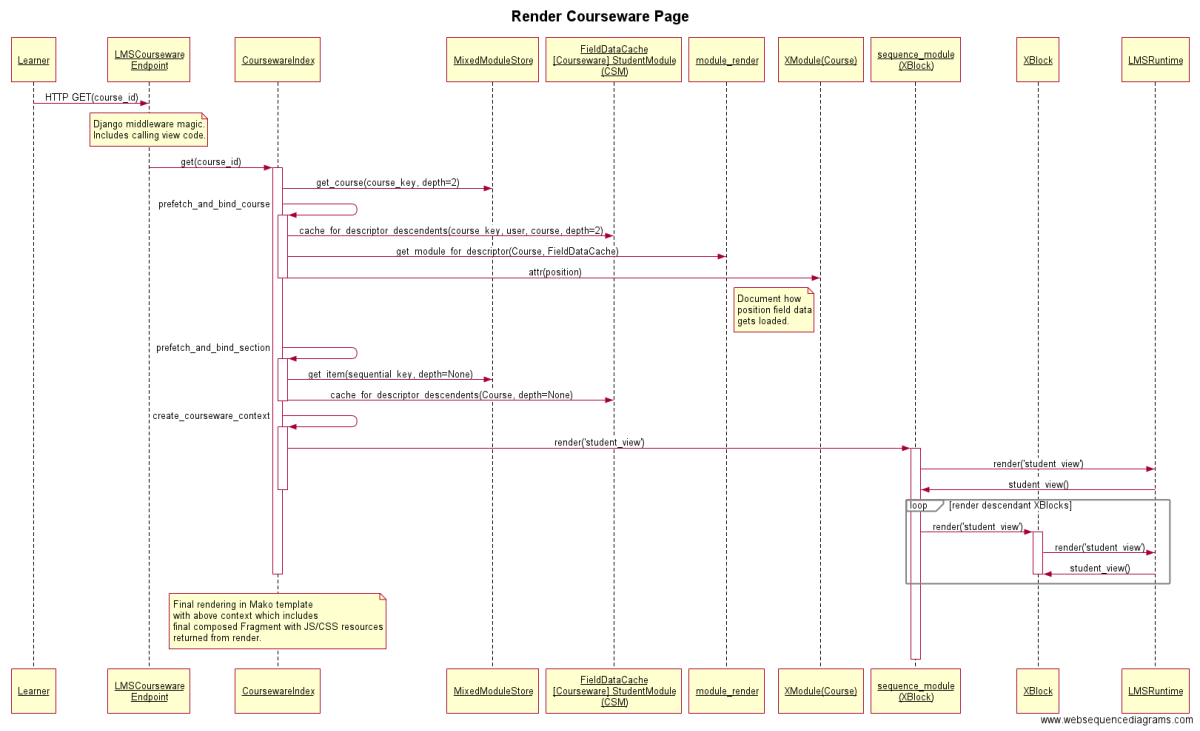
\includegraphics[width=\linewidth]{images/Render_Courseware_Page_Sequence_Diagram.png}
	\caption{Rendering of courseware using XBlocks}
	\label{Fig.1:Sequence diagram}
\end{figure}


\section{Testing and Installing Created XBlock}
\subsection{For Workbench}
We can test a xblock, while running with edX or workbench. We can install the xblock using following
commands and start as a local server, and open the browser to find the link for new xblock
\begin{enumerate}
\item Go to the root directory of new created xblock.
\item Type in the following commands\begin{center}\verb= pip install -e name of xblock=\end{center}
\item run the workbench as a local server using command python manage.py
runserver
\end{enumerate}


\subsection{For Open edX instance}
Clone the repository on our local machine. Testing this first on devstack is always recommended
\begin{enumerate}
\item Enter the shell of your devstack and execute :
\begin{center}\verb= sudo -u edxapp /edx/bin/pip.edxapp install /path/to/cloned/directory=\end{center}
\textbf{Note:} You need to point pip to the directory containing setup.py of our project.\newline For
example: If we cloned this repo in directory called\textbf{ /home/edx/advhtmlxblock} and
\textbf{/home/edx/advhtmlxblock/setup.py}is present then\textbf{ /home/edx/advhtmlxblock} is your
required path
\item (Re)start your LMS and CMS.
\item Login to studio as staff
\item Go to "Advanced Settings" in your course
\item Add word advancedhtml to list of "Advanced Modules"
\item Save changes
\item Advanced HTML component should be present in "Advanced" section in your course.
\end{enumerate}


%%%%%%%%%%%%%%%%%%%%%%%%%%%%%%%%%%%%


\chapter{Advanced HTML XBlock for Open edX platform}

\section{Features}
\begin{itemize}
	\item Full CSS Support
	\item JavaScript Suppport
	\item Live Preview HTML
	\item Code Indentation
	\item Code Folding
	\item Autocomplete Tags
	\item Autocomplete Brackets
\end{itemize}

\section{Installation}
Installation instructions are already covered in previous chapters(Creating an Xblock)\newline
\textbf{Special Note for Docker based devstack :}\newline
Since the docker based devstack has 2 separate containers for lms and studio, it is required that you
install this xblock in both the containers and then [re]start both lms and studio to see changes.
The workflow would look something like this :
\begin{enumerate}
	\item \verb= make studio-shell=
	\item Install xblock as mentioned before
	\item \verb=exit= from studio-shell
	\item \verb= make lms-shell=
	\item Install xblock as mentioned before
	\item \verb=exit= from lms-shell
	\item \verb=make studio-restart && make lms-restart=
\end{enumerate}

\section{Working}
AdvancedHTMLXBlock essentially extends raw HTML component of OpenEdx. This Xblock uses
the latest version of CodeMirror(5.38 as of June 2018). Editor is configured to enable code folding/
code indentation etc. All the html content received from the editor is then put into an iframe. The
height of the iframe is changed on changes in html content and iframe is styled so that it looks
virtually absent.

\section{Technical Details}
Fields :
\begin{enumerate}
\item \textbf{display\_name} : This is the name shown to user(course creator) in “Advanced” component
list in studio
\item \textbf{htmlcontent} : This is the actual htmlcontent that will be rendered to student in student\_view
\item \textbf{live\_preview}: This stores the live preview preference of each xblock
\item \textbf{unique\_id} : This is the id used in student\_view’s html to differentiate from other xblocks.
This is NOT the unique id generated by OpenEdx platform(also known as locator). This
unique\_id is used as id of iframe in html template. Since this is unnique to each
advancedhtmlblock, you can add multiple advanced html xblocks on same page.
\item Rest fields are just the required fields for the xblock to be used successful in lms and studio
and do not hold much of significance
\end{enumerate}
Functions :
\begin{enumerate}
\item \textbf{student\_view} : \\
This is the function called by LmsRuntime to render the xblock to students.
Since the xblock does not explicitly define author\_view, student\_view is used as
author\_view. On the first run, this will generate unique\_id using uuid library. This id is
passed to student\_view template everytime student\_view is called. The student\_view is
nothing but a simple iframe with NO content inside it initially. Javascript will ask for
htmlcontent once it is initialized. Javascript queries the htmlcontent via AJAX and the
response is JSON. This htmlcontent is then written into iframe by javascript. Once the
content loads inside the iframe, height required for iframe is calculated and then that height
is set to the iframe rendering as if the iframe is absent.
\item \textbf{studio\_view} : \\
This is the editor panel that is shown to course creator in studio after “edit”
button is clicked. The function adds all the requrired CSS and JavaScript required for
CodeMirror to work properly. The interface of studio\_view also consists of a live preview
panel and Advanced Settings panel. Advanced Settings panel allows course creator to hide
live preview panel and change display name of xblock.
\end{enumerate}

\section{Screenshots and Source Code}
\begin{itemize}
\item The screenshots of our Workbench along with the editor are provided as mentioned below
\begin{center}\textbf{[See Figures 9-11 in the “Figures and Screenshots” section.]}\end{center}
\item The screenshots of our Advanced HTML XBlock in our running instance of Open edX are
provided as mentioned below:
\begin{center}\textbf{[See Figures 12-20 in the “Figures and Screenshots” section.]}\end{center}
\item The source code of our Advanced HTML XBlock is available on our github repository as
mentioned below:\newline
\begin{center}[\url{https://github.com/ashutoshbsathe/AdvancedHTMLXBlock}]\end{center}
\end{itemize}

\section{Testing} 
We have tested our xblock to see if we can include multiple xblock in a unit, move/copy an xblock from one unit to another unit, importing/exporting a course with our xblock \newline
We have also tested if all HTML tags/CSS styling and JS is working \newline 
JavaScript has one restriction that it cannot access the topmost window for security reasons. This is tested and it works good so far. \newline\newline
Full test report can be found here : \newline 
\begin{small}
\url{https://docs.google.com/spreadsheets/d/11XM9PDOGZzXspLcwYCWpo9gYTPaiNUo_MKtTmz873sM/edit#gid=0}
\end{small}


\section{Issues and solutions}
\begin{itemize}
	\item \textbf{Broken codemirror features :}\newline
The codemirror source was stripped down to include only the features we need. So it was
tricky to include them in the xblock. However, understanding codemirror code helped us
include it nicely
	\item \textbf{CodeMirror conflicts :}\newline
This issue was not faced on local workbench, we faced this issue when we integrated our
xblock in devstack. The problem was studio and lms already have a version of CodeMirror
loaded with them, so loading our version alongside with it was going to be a problem. We
modified a bit of codemirror source code to make it work in “browser only” mode.
This also brings us to the important conclusion about fragment API. The xblock’s html, CSS
and JavaScript is rendered into a fragment which is then rendered by studio/lms. The catch
is the fragments are not separate from each other. That means one fragment’s CSS/JS can
interfere with another fragment’s CSS/JS and in usual, can interfere with main CSS and JS
used by page. This is potentially dangerous as it can execute some bad code which can break
the entire page.
	\item \textbf{JavaScript Security concerns :}\newline
While our xblock can allow you to add html and css to beautify your course, it will also
allow you to add javascript to your course content to make it interactive. The security
concern was scope of javascript. The scope of javascript must be limited to iframe and
iframe ONLY. Xblock’s javascript in no way should be allowed to access toplevel window.
This was fixed by “sandboxing” the iframe and allowing limited javascript functionalities.
Check out this for more info :\newline
\begin{center}[Commit hash : 3a9d7e3890aa3da834be1d335f4ab799b6629cf3]\end{center}
\begin{center} OR Click below \end{center}
\begin{center}
\begin{tiny}\url{https://github.com/ashutoshbsathe/AdvancedHTMLXBlock/commit/3a9d7e3890aa3da834be1d335f4ab799b6629cf3}\end{tiny}
\end{center}
\end{itemize}
\chapter{Conclusion}
Delivering the course content to learners in better ways is most important in any educational system.
In present online education system, the successful completion rate of a course is very less.
XBlocks can be used to provide the  interface to deliver the course content in better ways to
attract the learners and deliver courses in a modular way.
\newline
\newline
Our Advanced HTML Xblock provides a great platform to increase the  interactivity of the courses and
enhance the learning experience of the students. It is a great tool for text-intent course content
creators as it provides them with total control over the course content. In contrast to the present text
editor in edx-platform, functionalities of our Xblock are merely limited to the imagination of the
course author. It will be a great addition to the current working lists of Xblocks present in Open edX
and will considerably boost the user experience.
\chapter {Future Work}
\begin{enumerate}
\item \textbf{Auto-complete feature in the editor :} \newline
Currently, this feature is absent in our version of CodeMirror implemented in the Advanced
HTML Xblock . It can be implemented in the future where a user will be shown a list of
options of the probable keywords on the basis of a keystroke.
\newline\newline  \textbf{Reference:} [\url{https://codemirror.net/demo/complete.html}]
\item \textbf{Setting a common CSS for an entire course :} \newline
Presently, if a course author wants to have a unified visual theme for all the content in a particular
course, he/she would have to manually apply the CSS style to each and every unit in the html
code. To make this easier we can have a common CSS file which will be automatically
fetched and imported for every unit in that course as per the settings of the course. One
possible way of implementing it would be making changes on the Django backend of that
particular course to fetch that CSS file from the \textbf{ “Files \& uploads”} section present for every
course in Open edX platform.
\item \textbf{Additional settings in the Xblock :}\newline
At present our Xblock has two options in the settings tab. Display name and Live preview
toggle. Some other features that can be added are :
\begin{itemize}
\item An option for selecting a dark/light theme for the editor to enhance the user experience
even more.
\item Enable a draggable partition interface so that users can adjust the size of the editor
window and the preview windows as desired.
\end{itemize}
\end{enumerate}
\chapter{Figures and Screenshots}

%\begin{figure}
 % 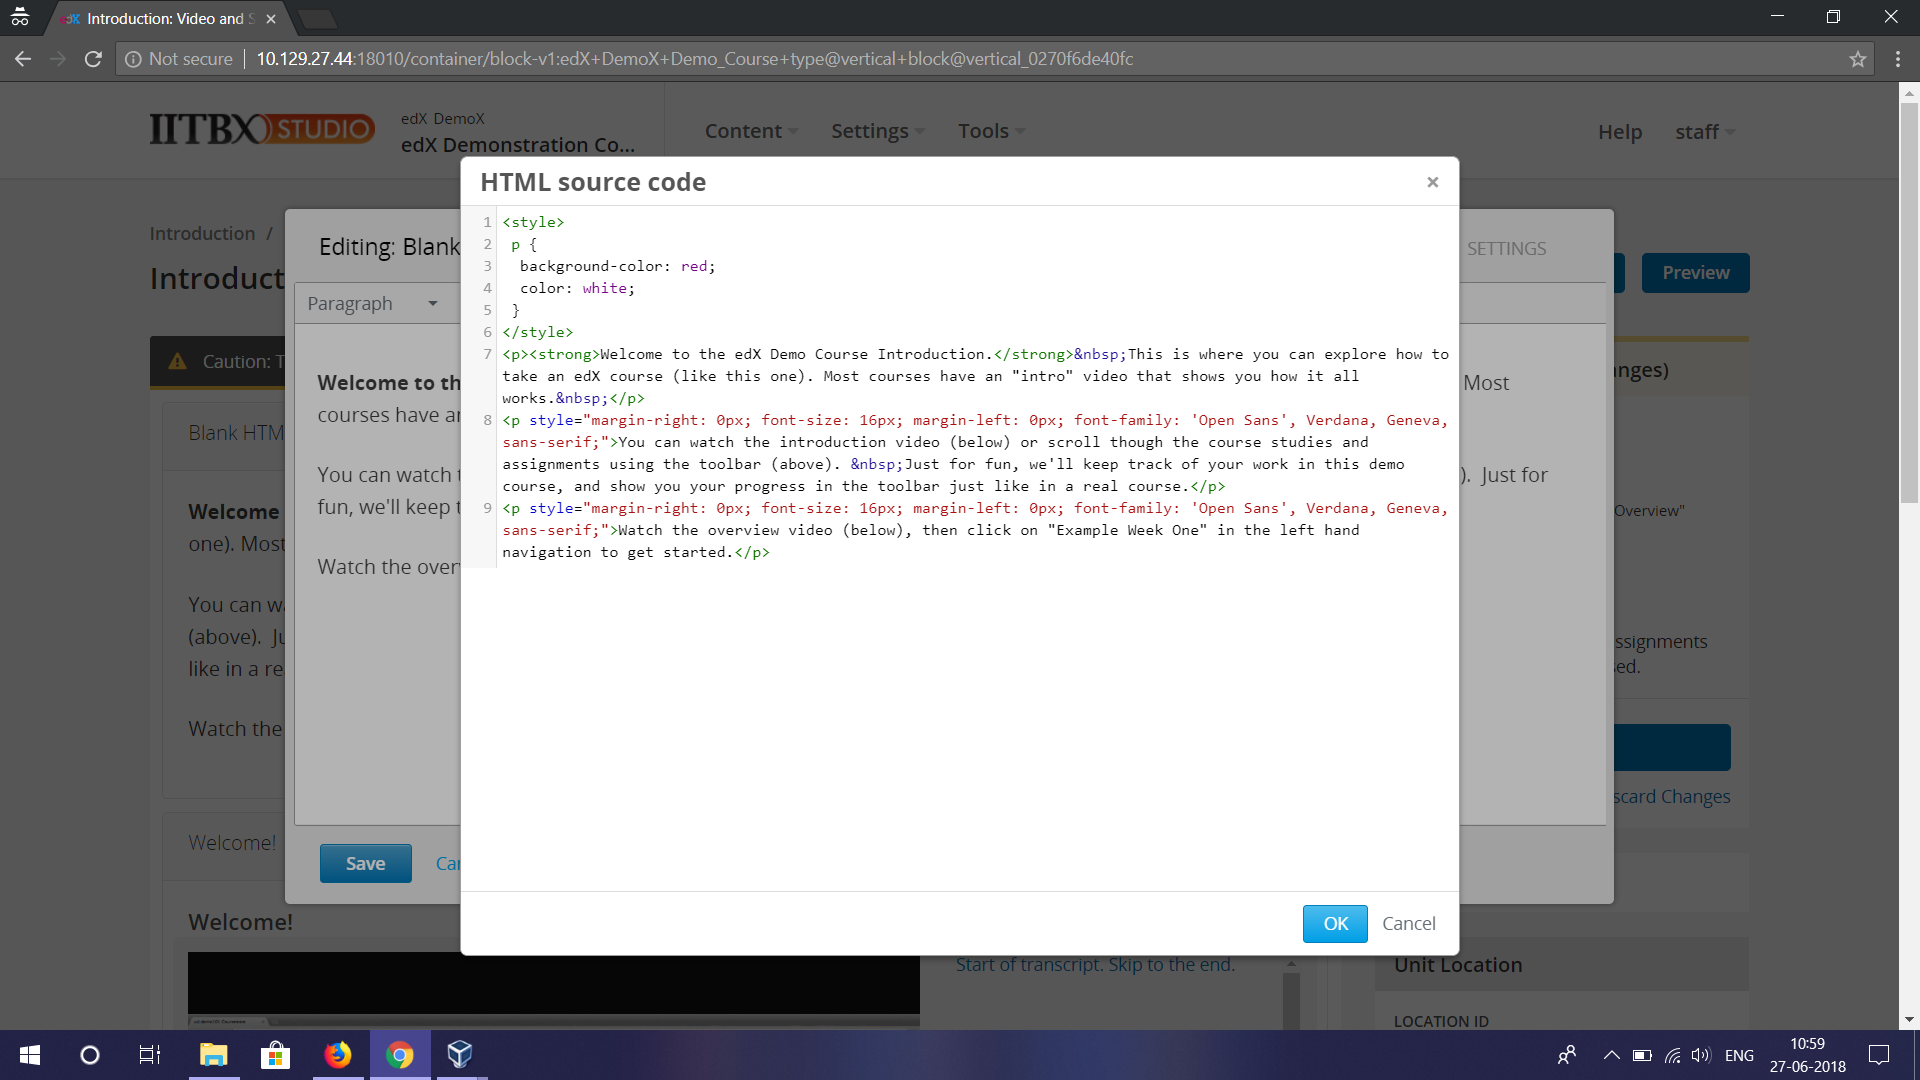
\includegraphics[width=\linewidth]{images/issue_0.png}
  %\caption{Adding CSS style tag manually}
  %\label{Fig.1:Issue_1}
%\end{figure}

\begin{figure}[ht]
  \centering
  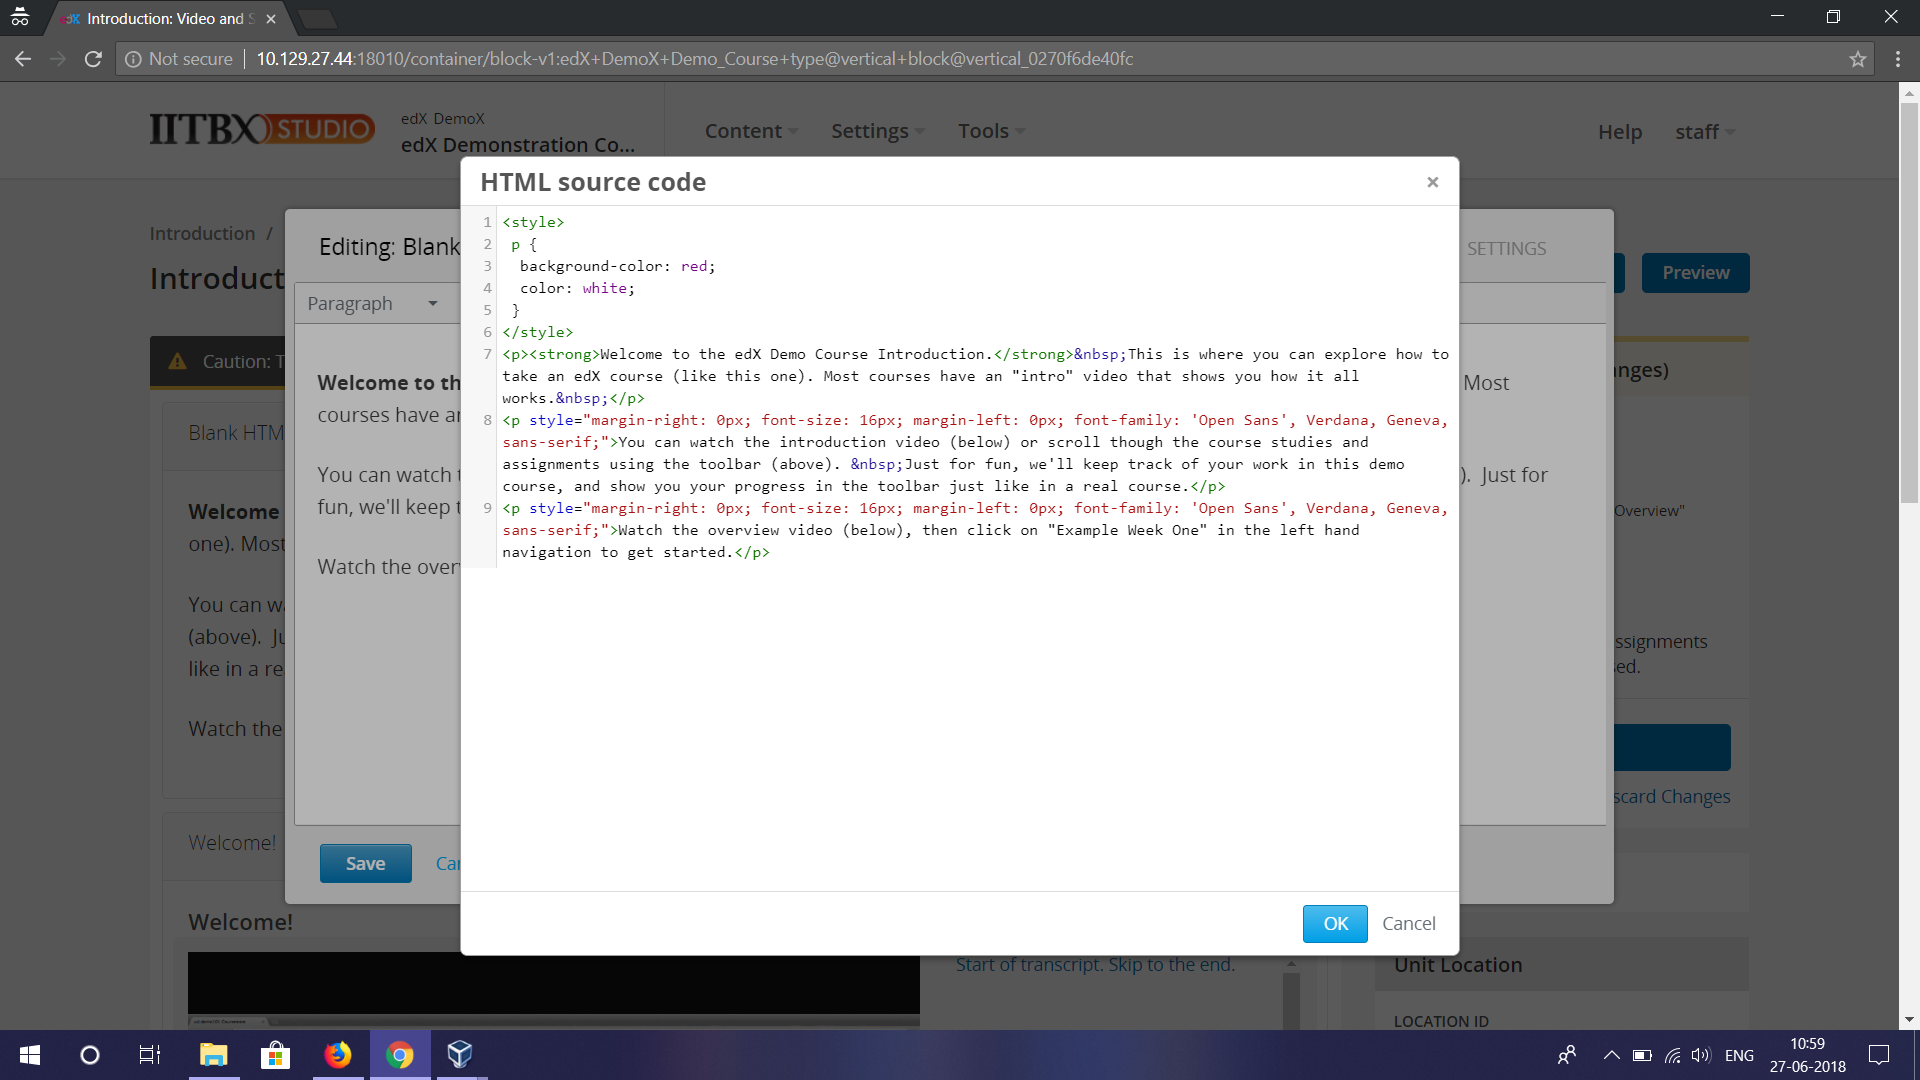
\includegraphics[width=\textwidth]{images/issue_0}
  \caption{Adding CSS style tag manually}

  \vspace*{\floatsep}

  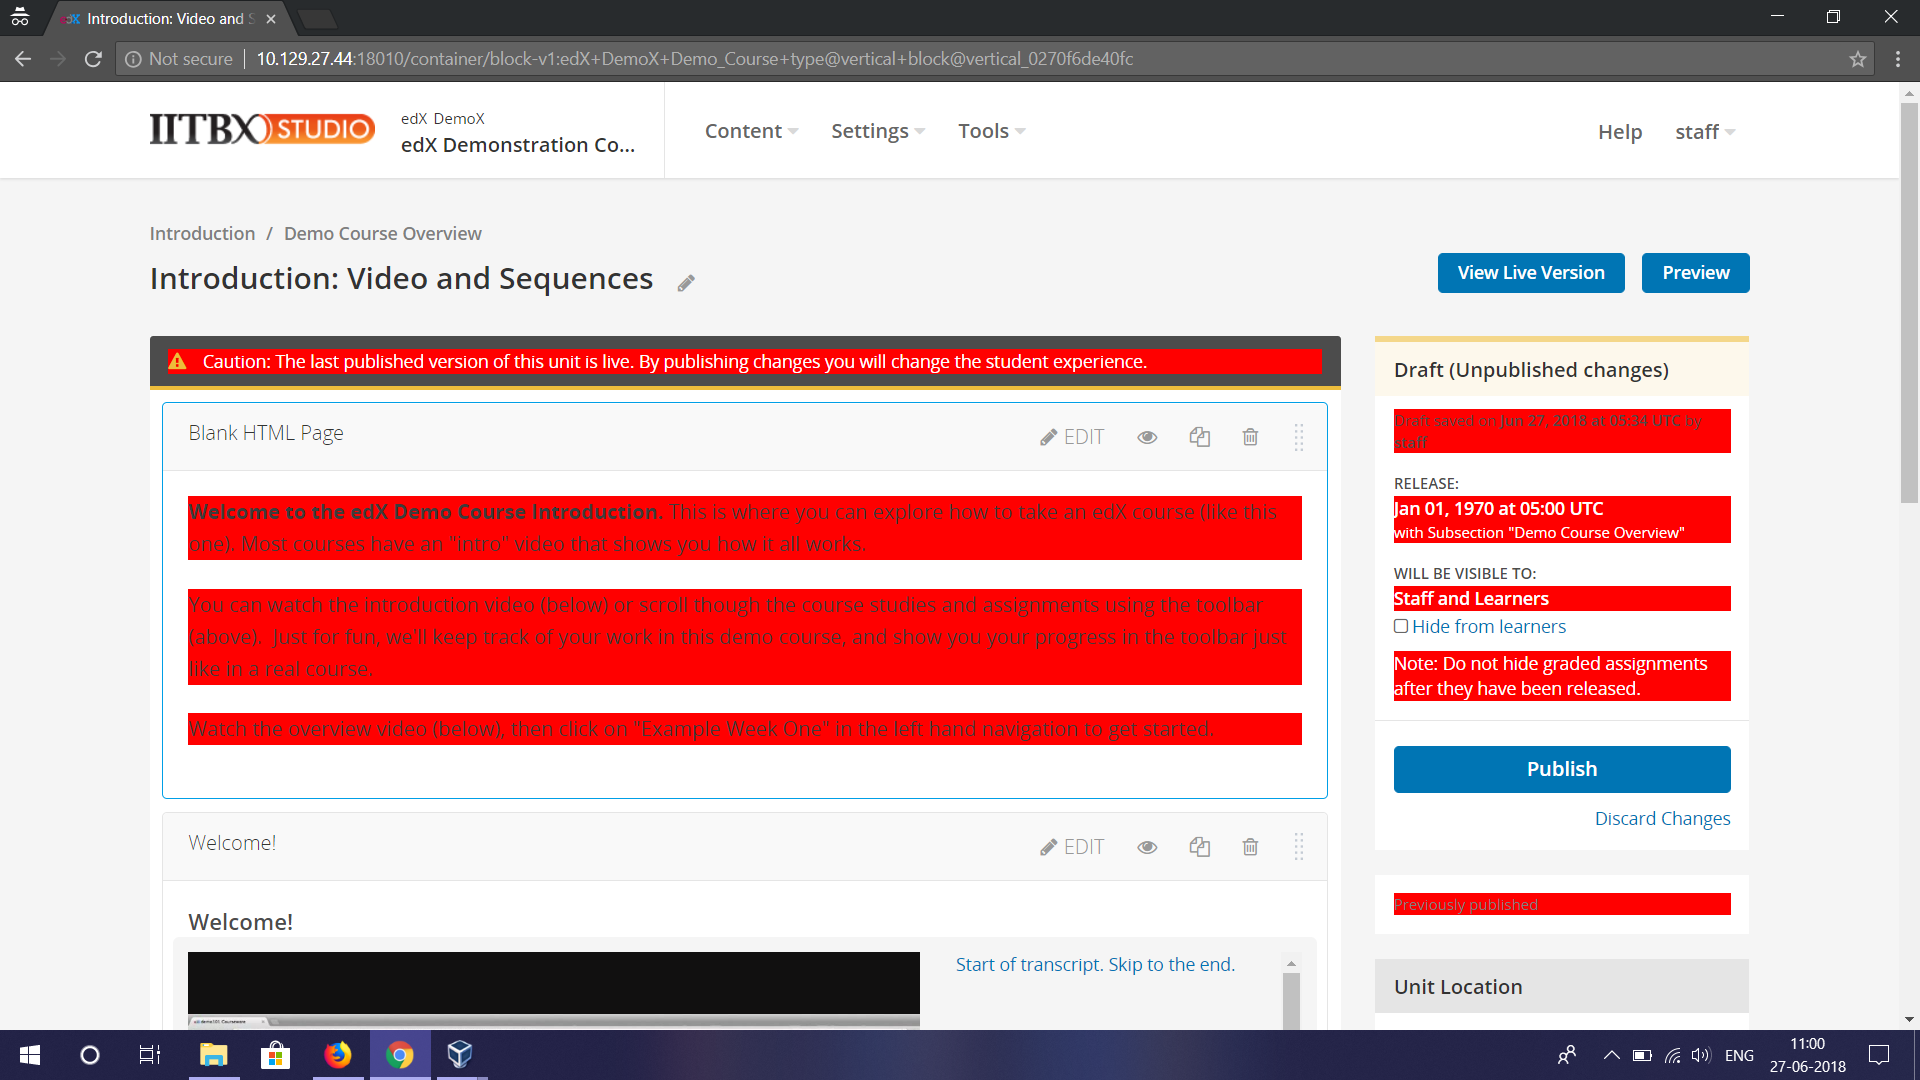
\includegraphics[width=\textwidth]{images/issue_1}
  \caption{CSS gets spilled all over page}
\end{figure}

\begin{figure}[ht]
  \centering
  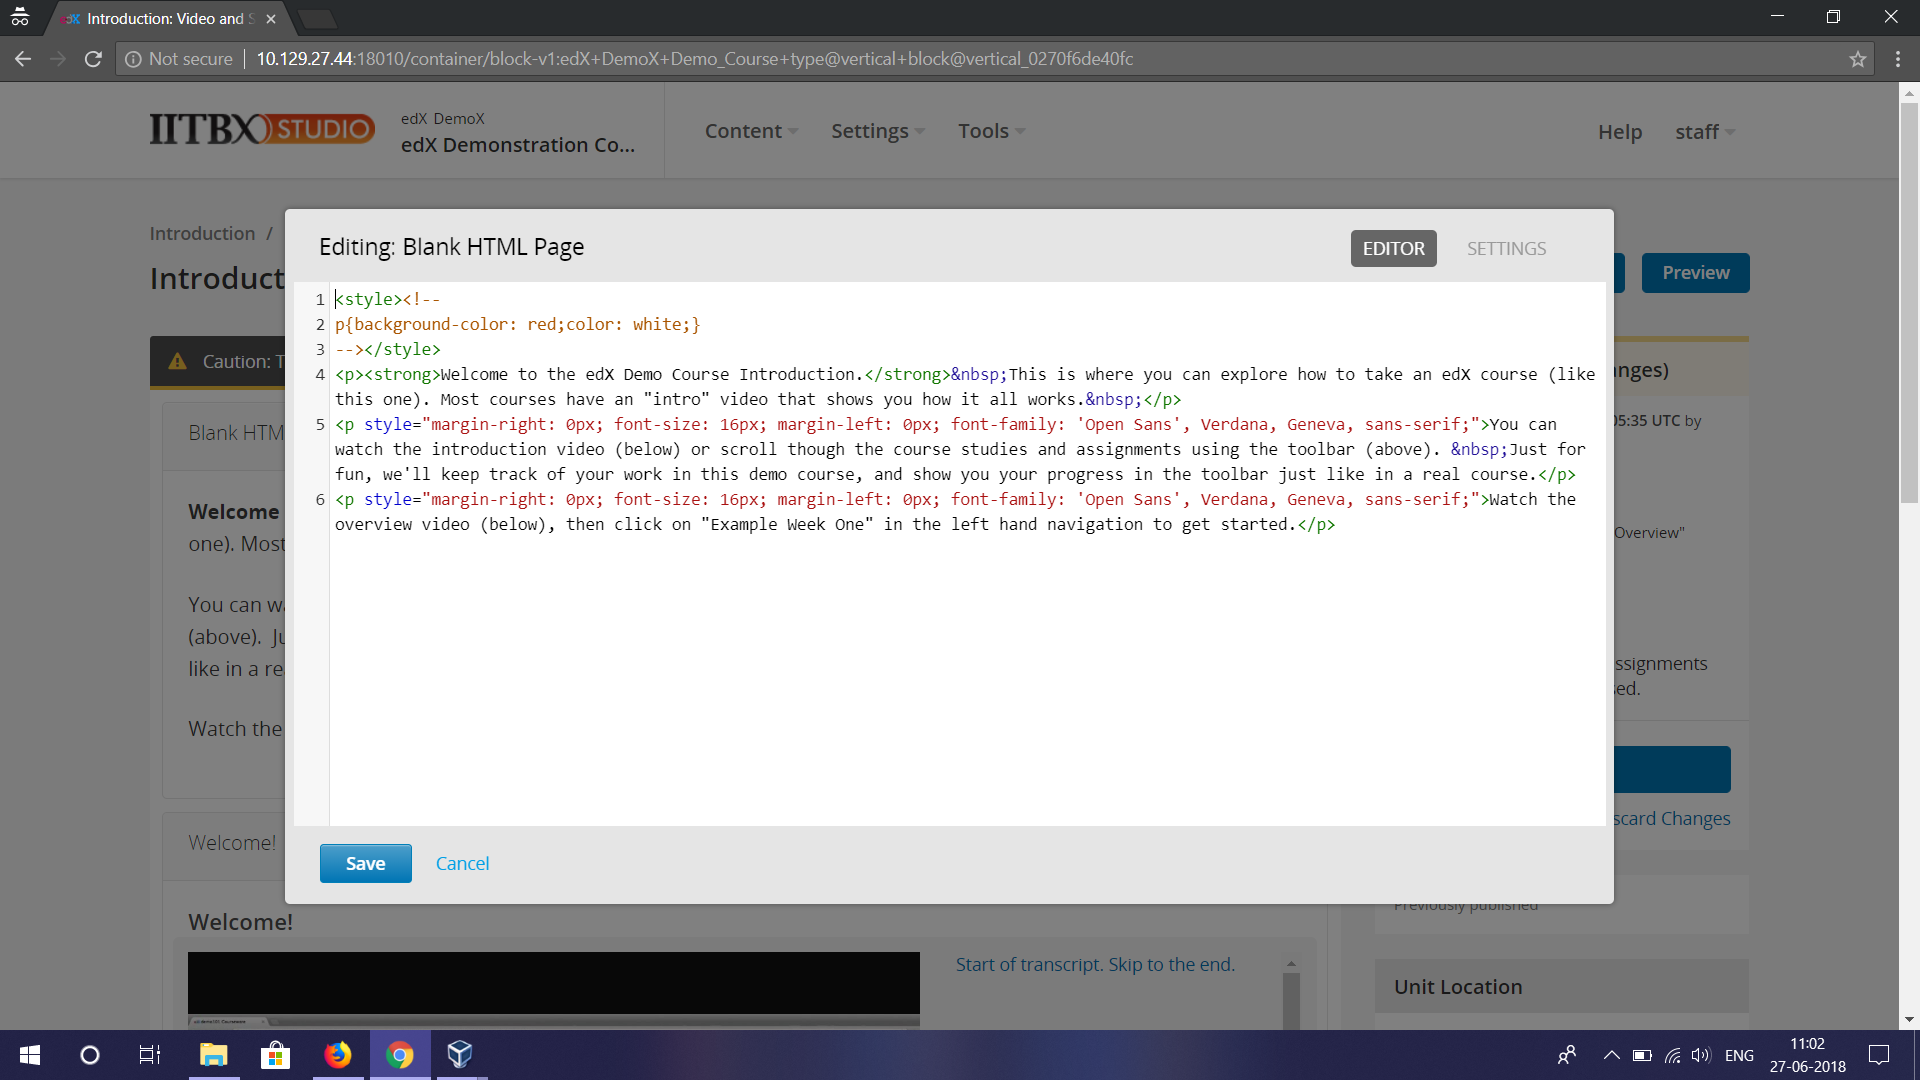
\includegraphics[width=\textwidth]{images/issue_2}
  \caption{Indentation not preserved on re-editing}

  \vspace*{\floatsep}

  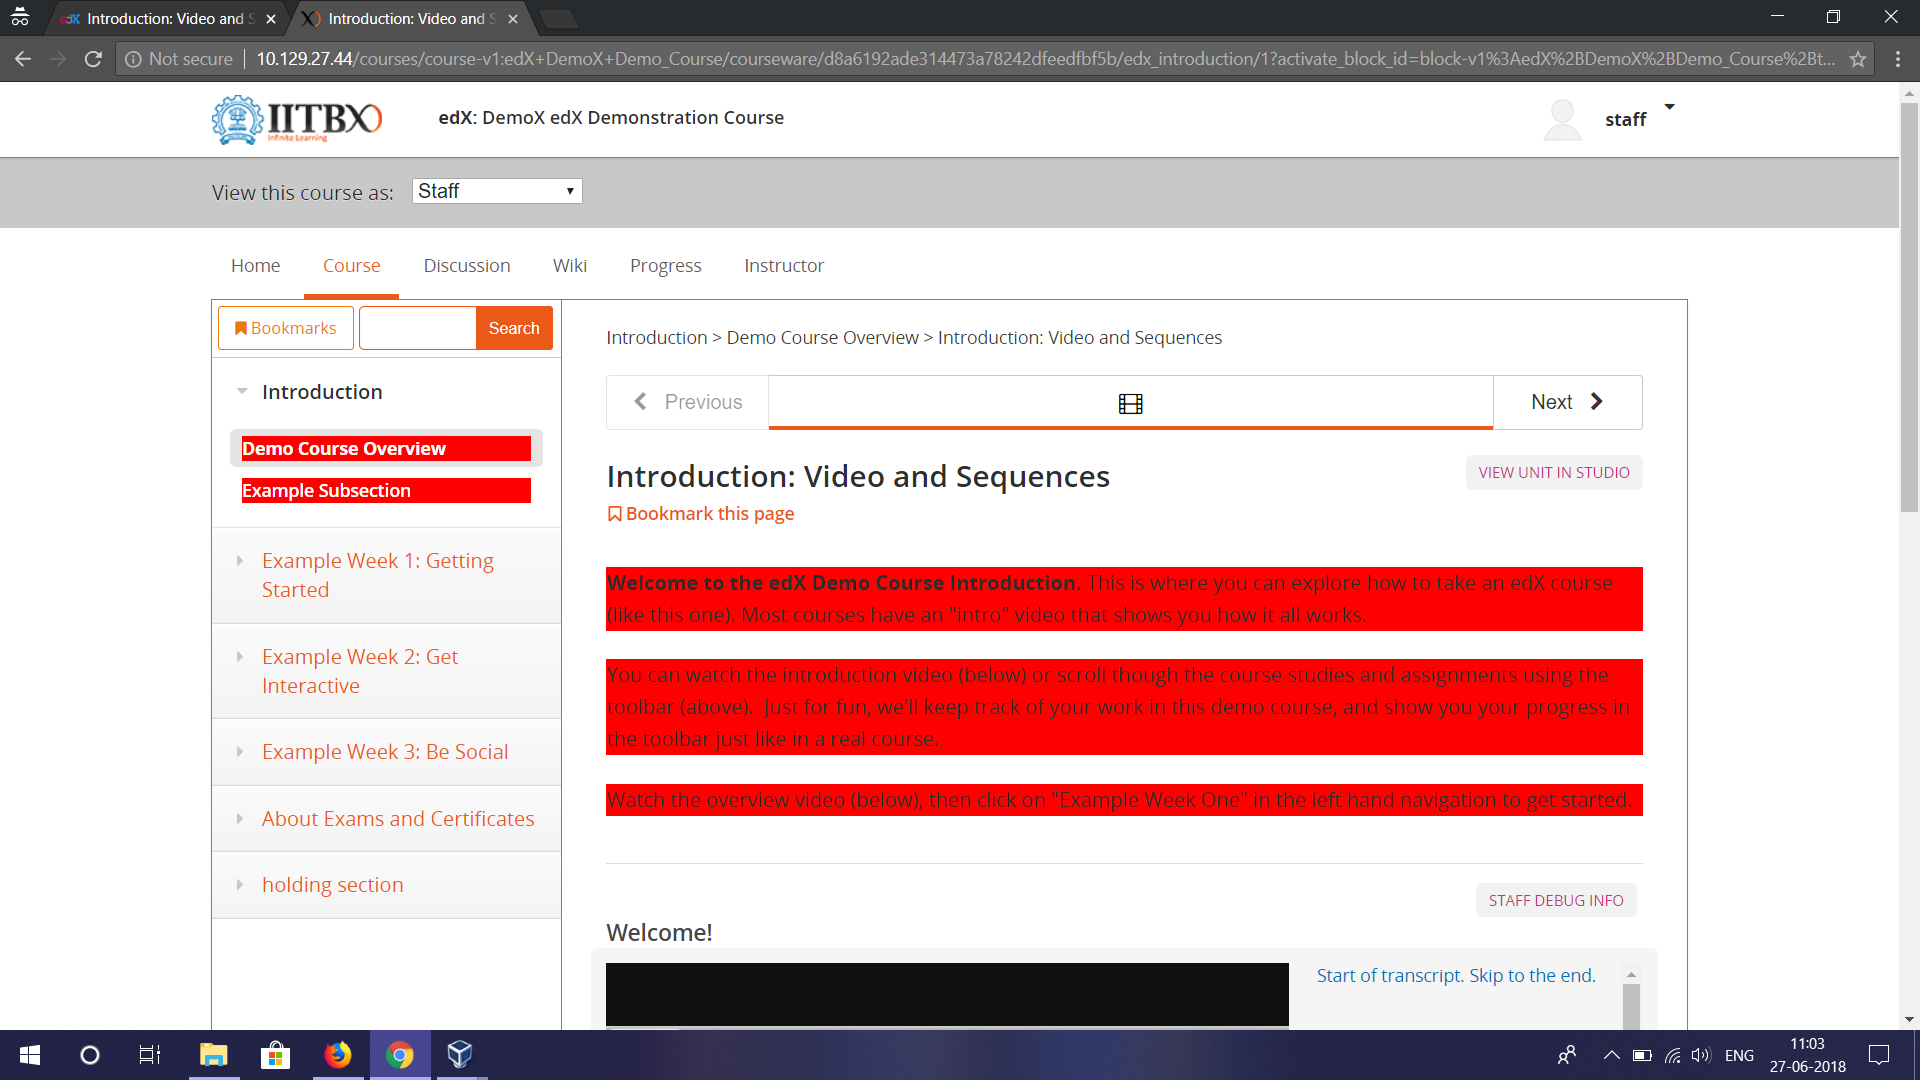
\includegraphics[width=\textwidth]{images/issue_3}
  \caption{CSS spilled all over page in LMS}
\end{figure}

\begin{figure}[ht]
  \centering
  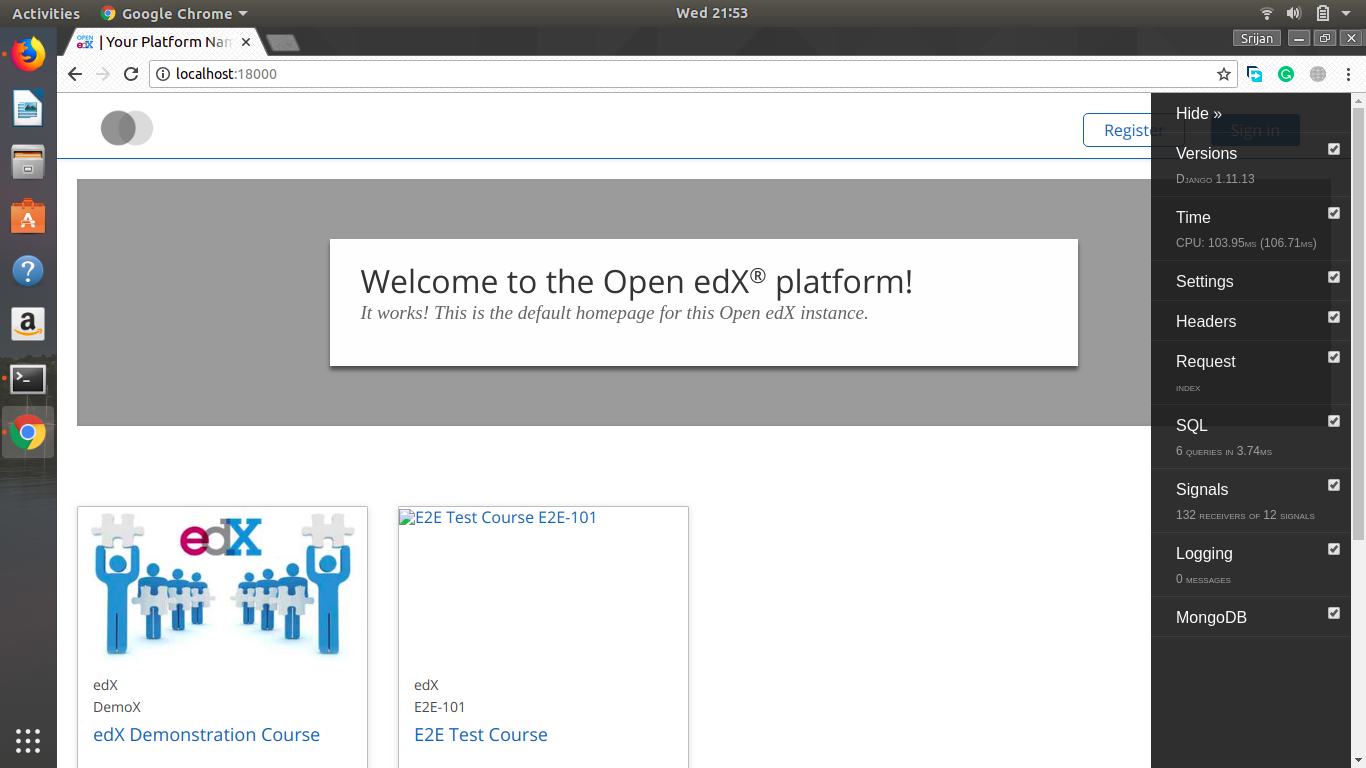
\includegraphics[width=\textwidth]{images/devstack_0}
  \caption{LMS landing page}

  \vspace*{\floatsep}

  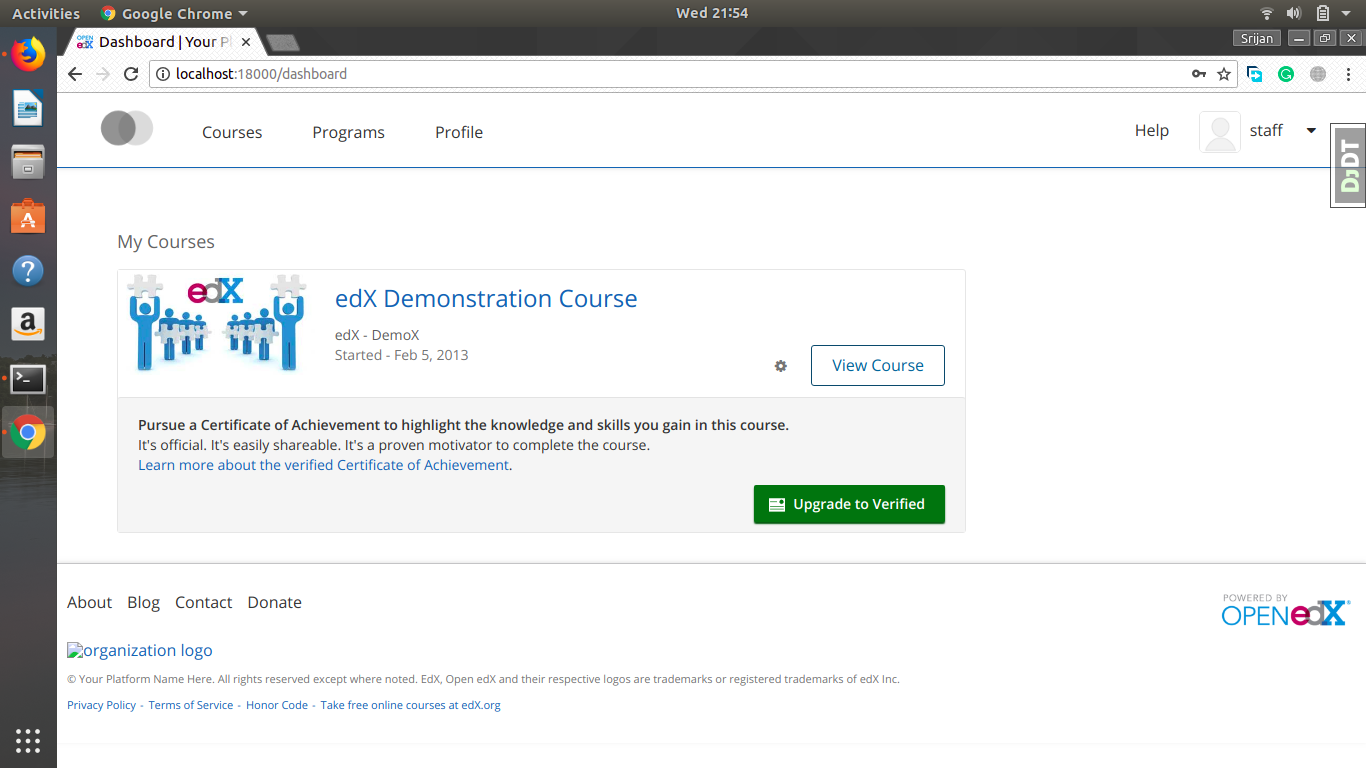
\includegraphics[width=\textwidth]{images/devstack_1}
  \caption{Staff login in CMS}
\end{figure}

\begin{figure}[ht]
  \centering
  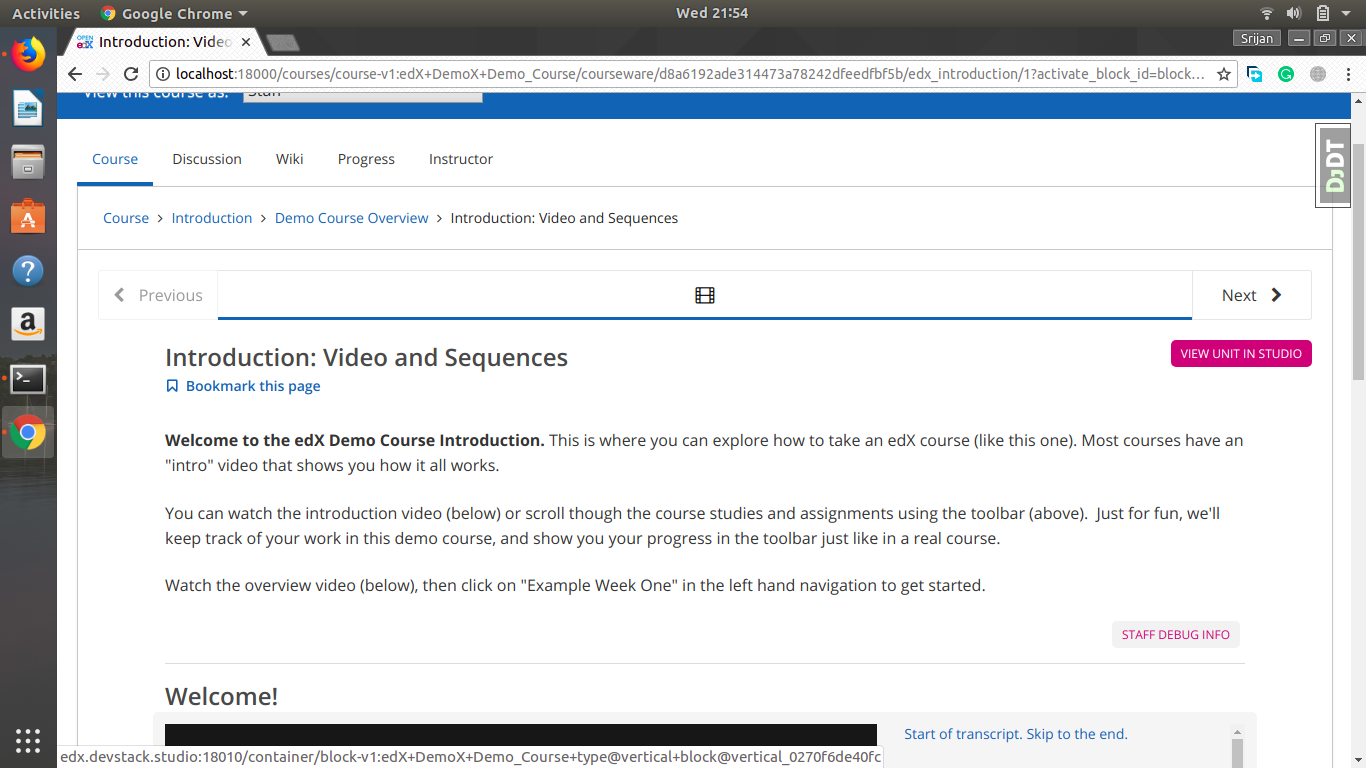
\includegraphics[width=\textwidth]{images/devstack_2}
  \caption{Viewing course in LMS}

  \vspace*{\floatsep}

  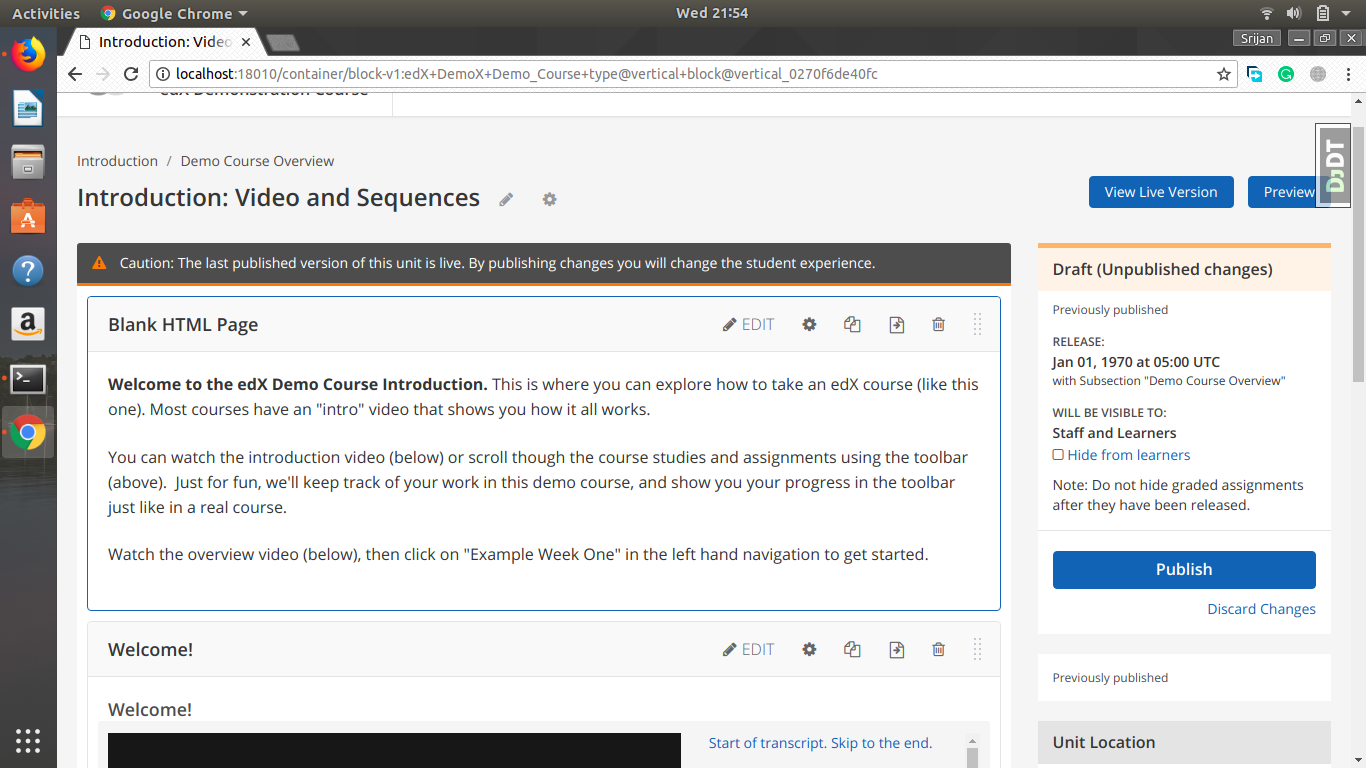
\includegraphics[width=\textwidth]{images/devstack_3}
  \caption{Viewing course in CMS}
\end{figure}



\begin{figure}[ht]
  \centering
  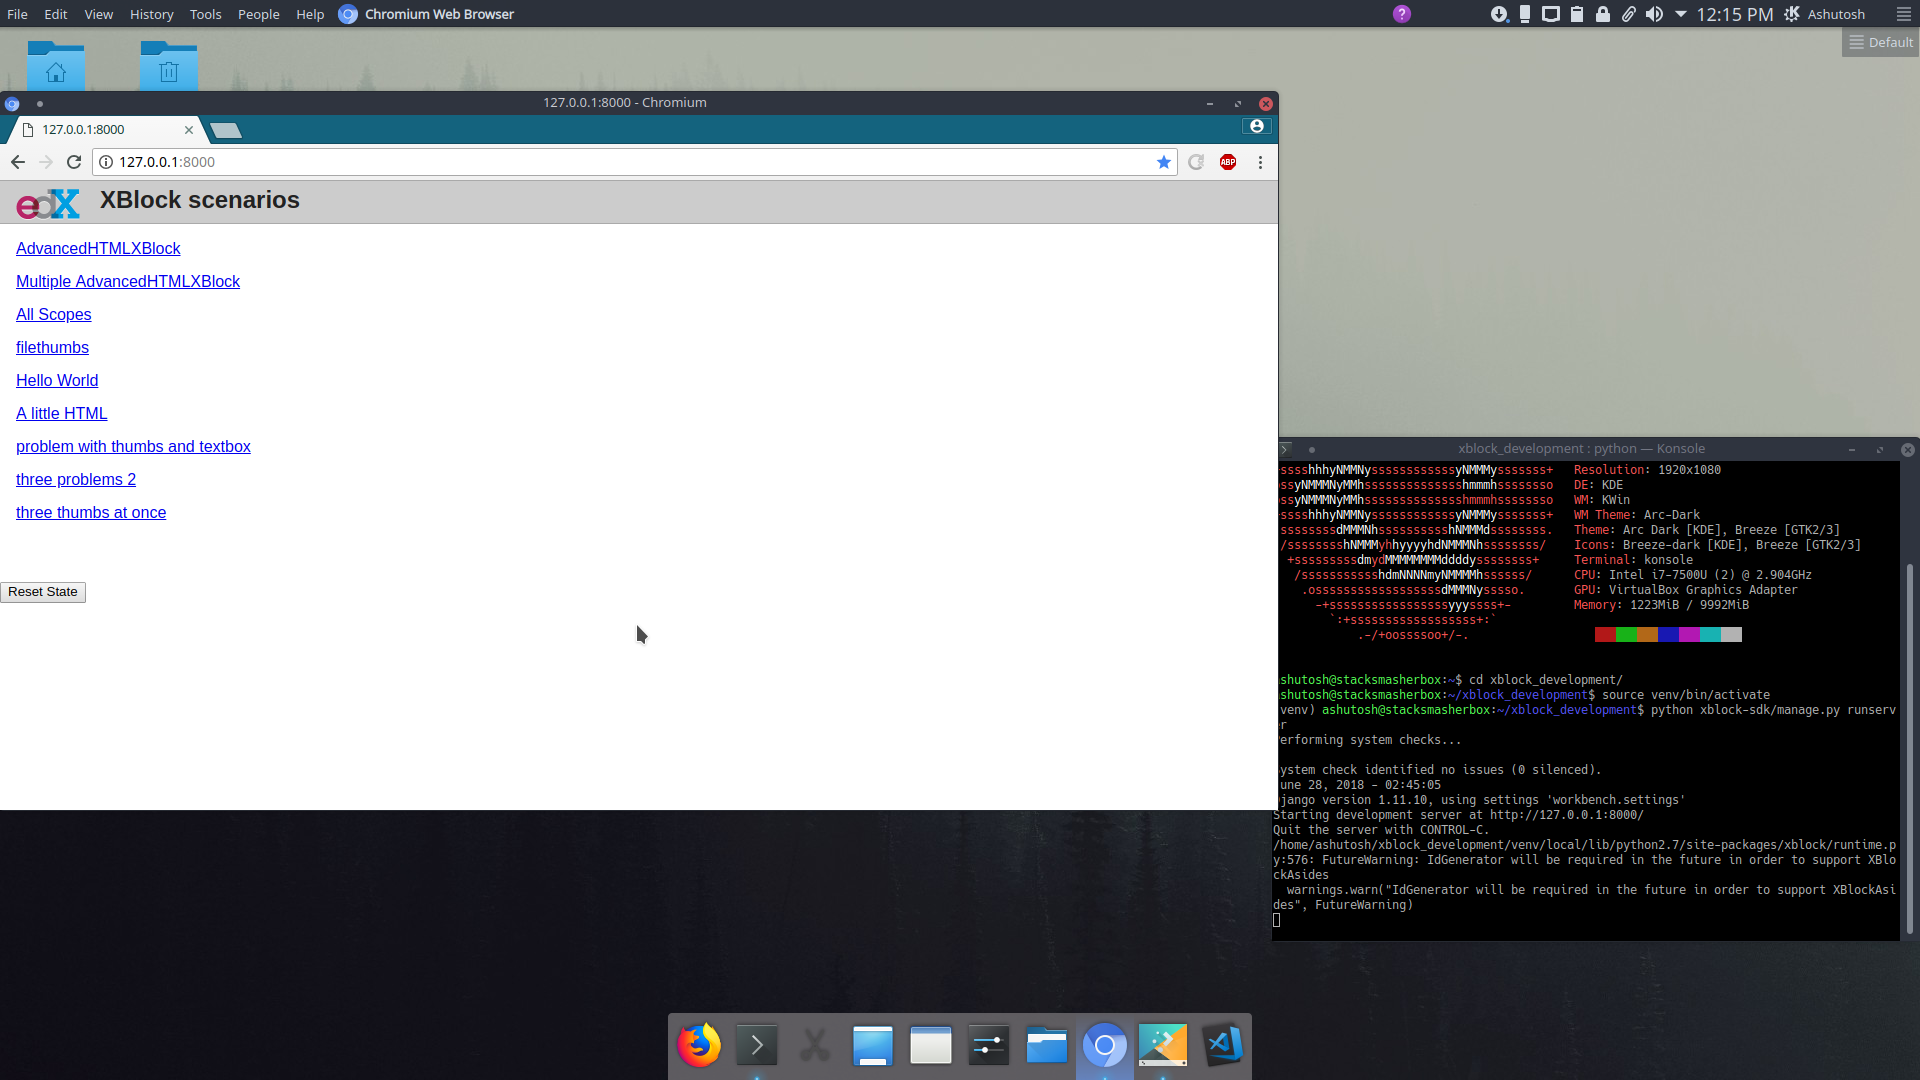
\includegraphics[width=\textwidth]{images/workbench_0}
  \caption{Landing page of workbench}

  \vspace*{\floatsep}

  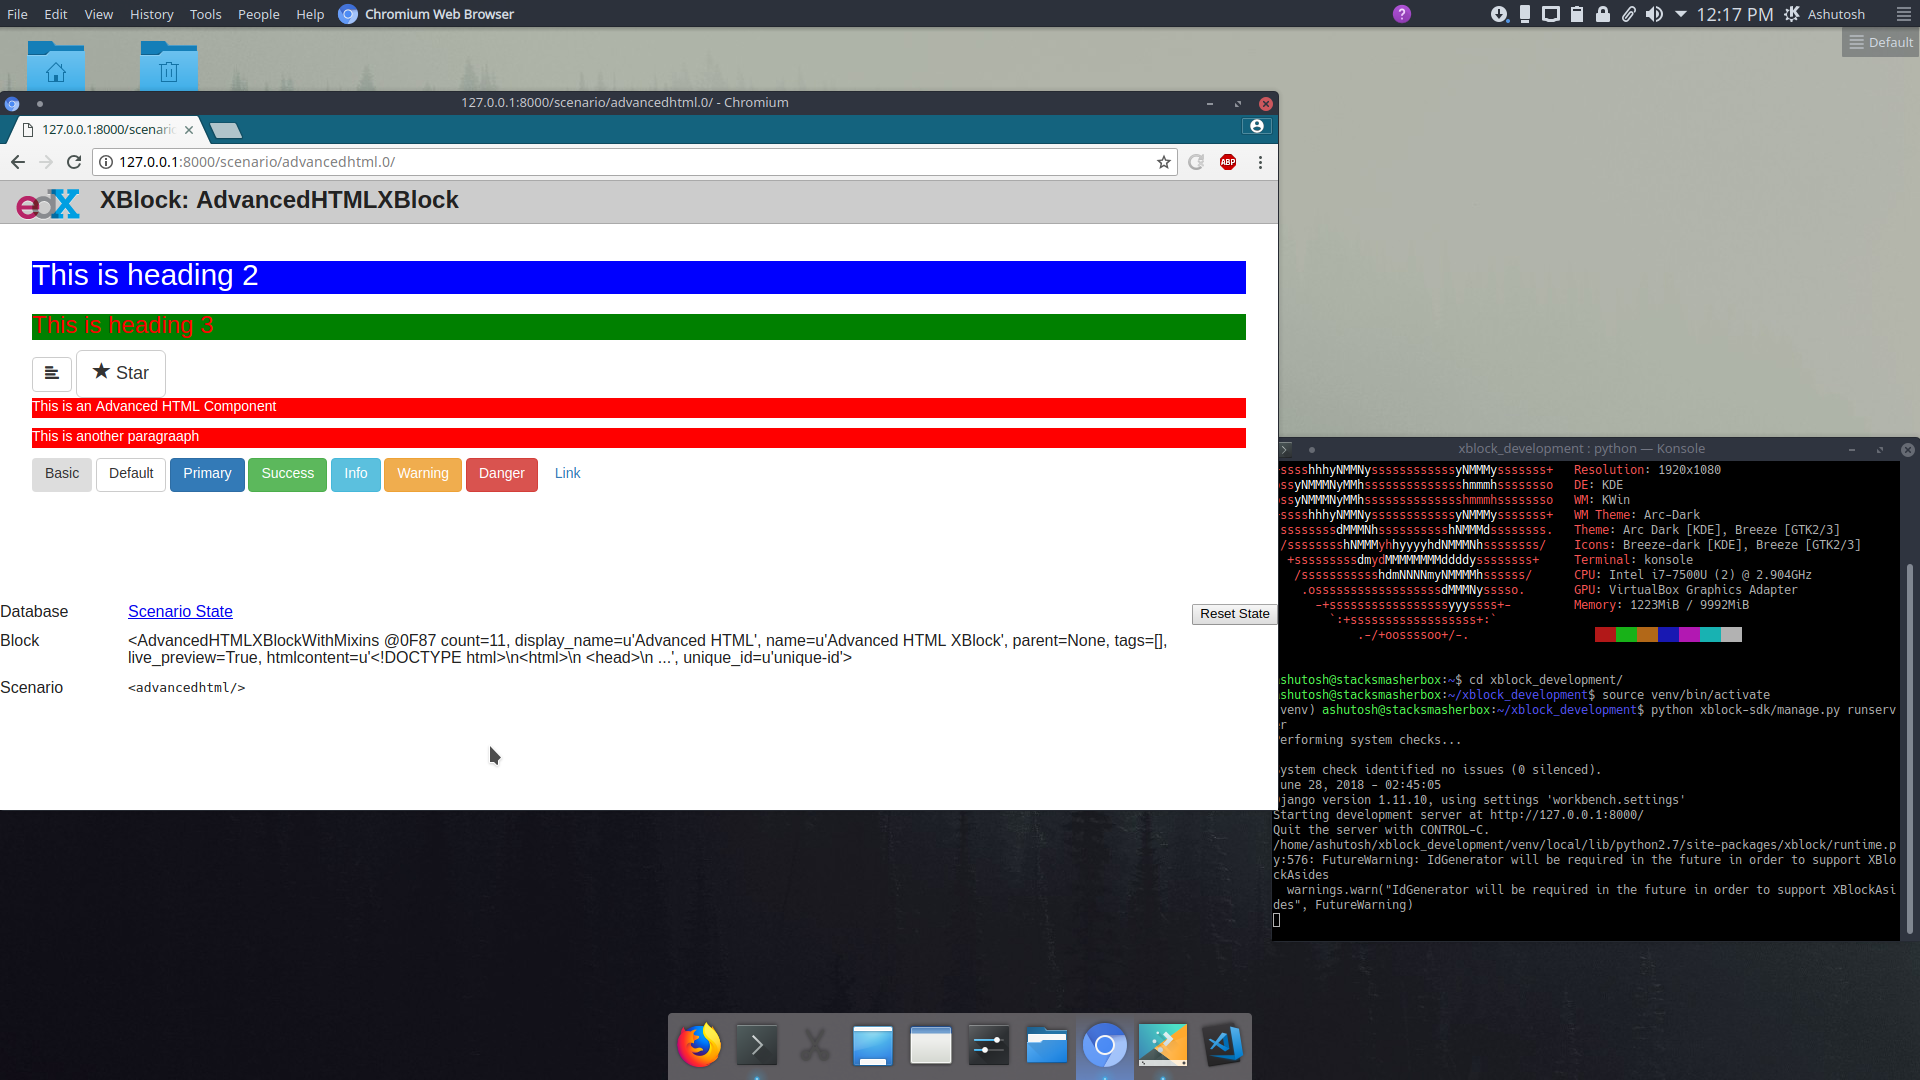
\includegraphics[width=\textwidth]{images/workbench_1}
  \caption{Viewing single xblock scenario}
\end{figure}

\begin{figure}[ht]
  \centering
  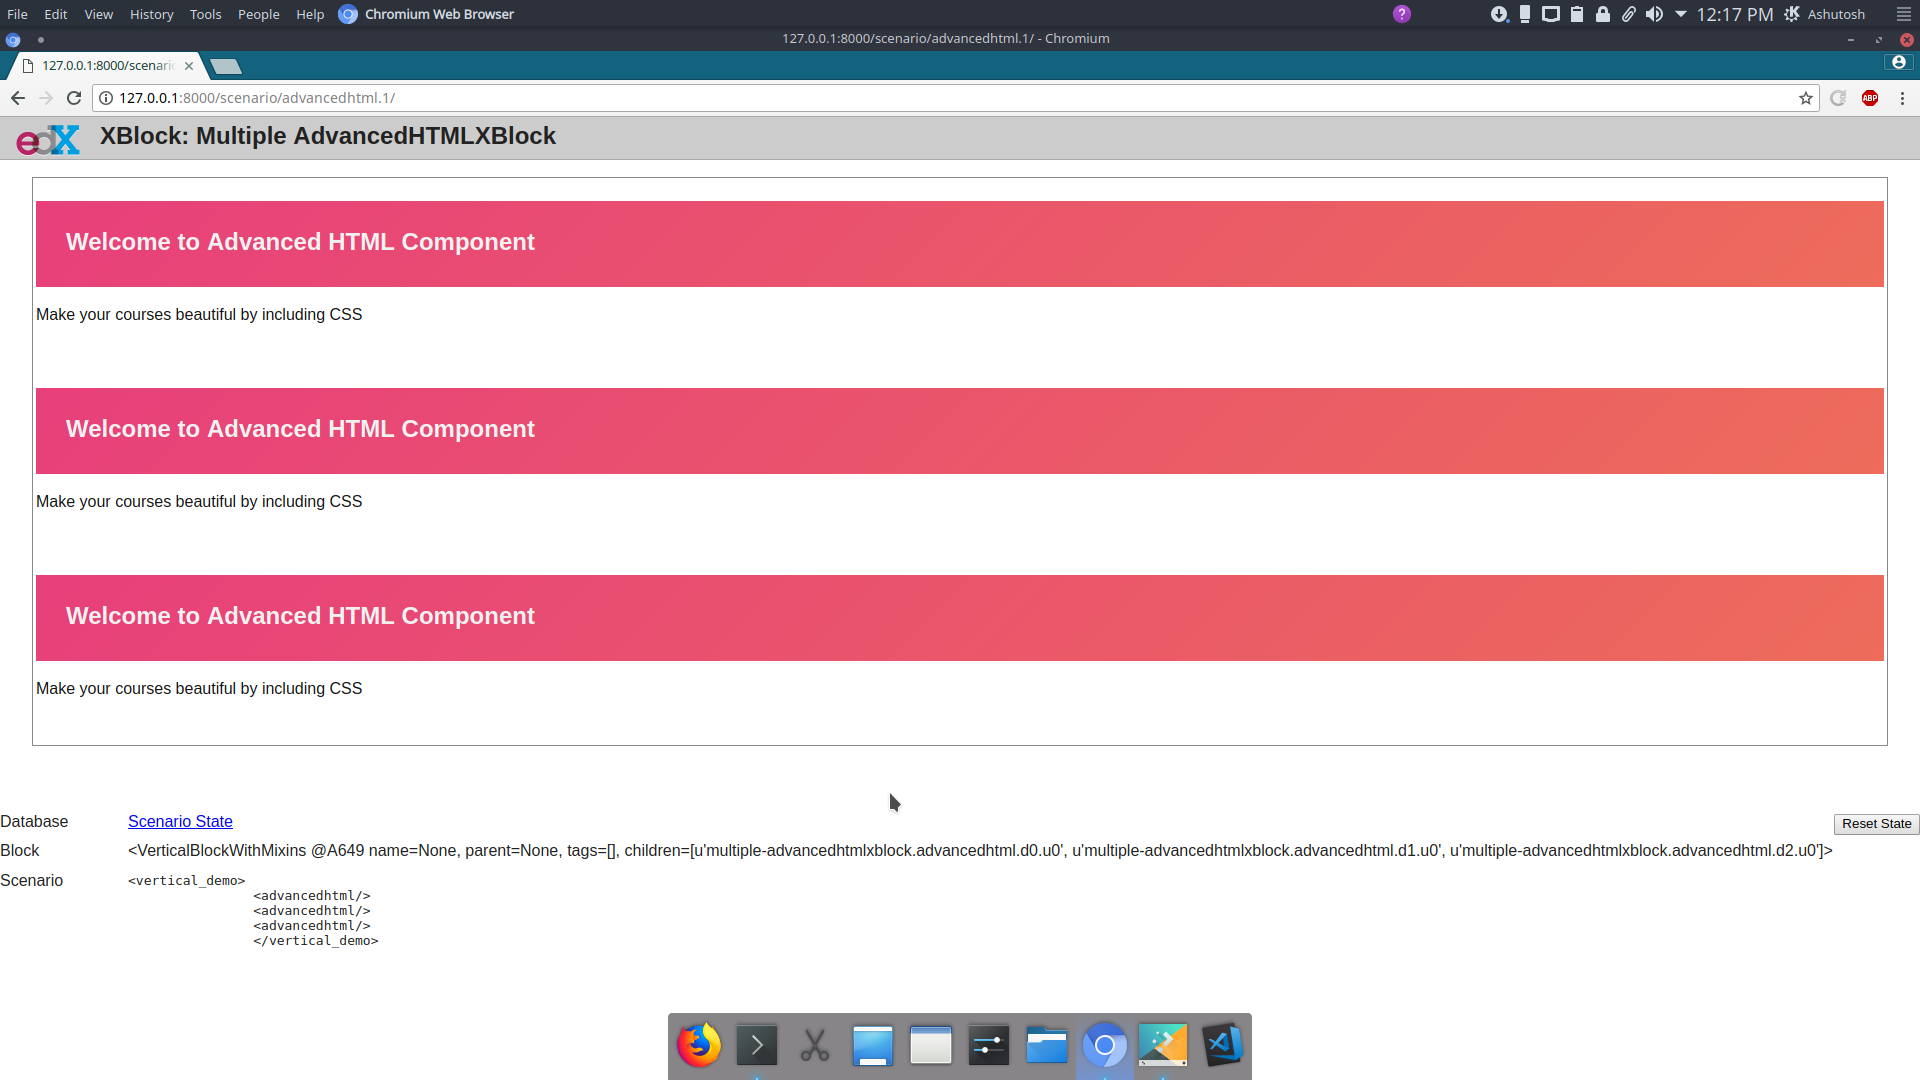
\includegraphics[width=\textwidth]{images/workbench_2}
  \caption{Viewing multiple xblocks senario}

  \vspace*{\floatsep}

  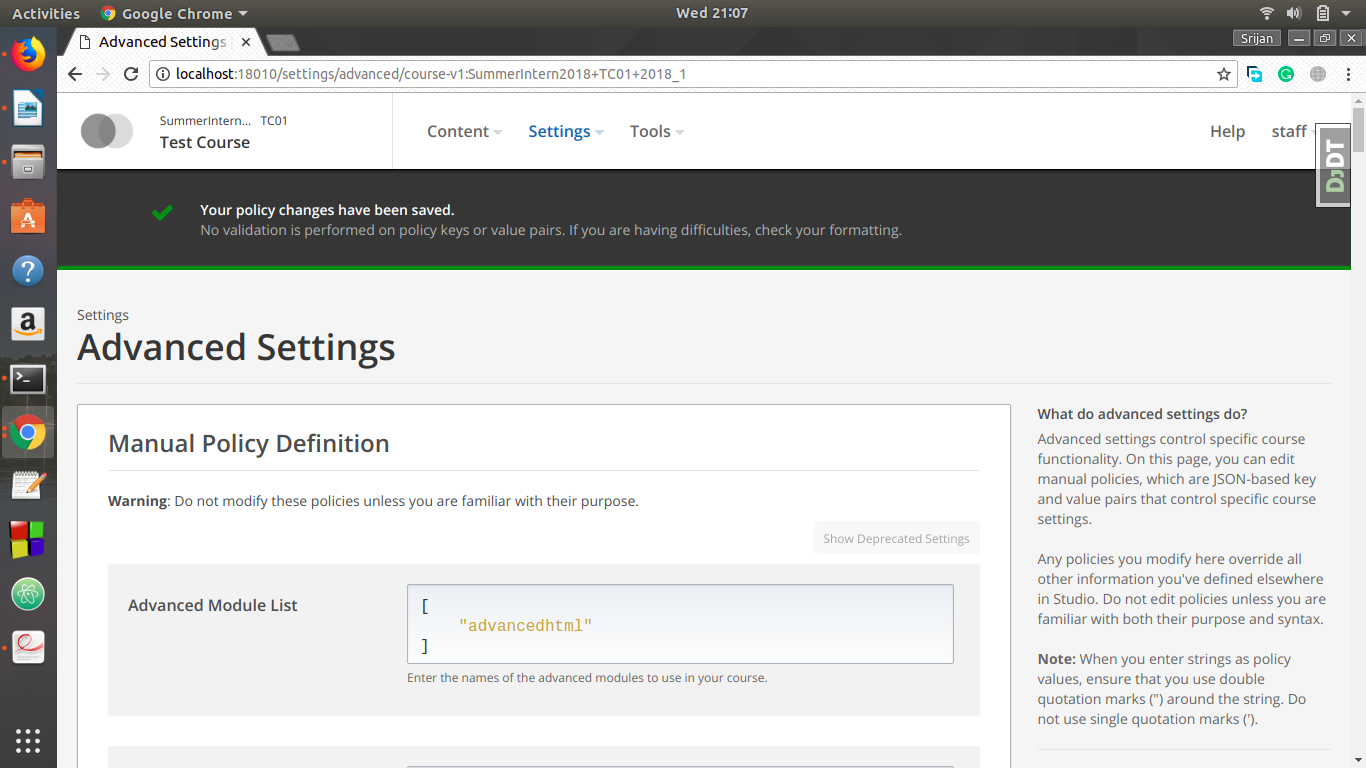
\includegraphics[width=\textwidth]{images/demo_0}
  \caption{Adding xblock name in advanced settings}
\end{figure}


\begin{figure}[ht]
  \centering
  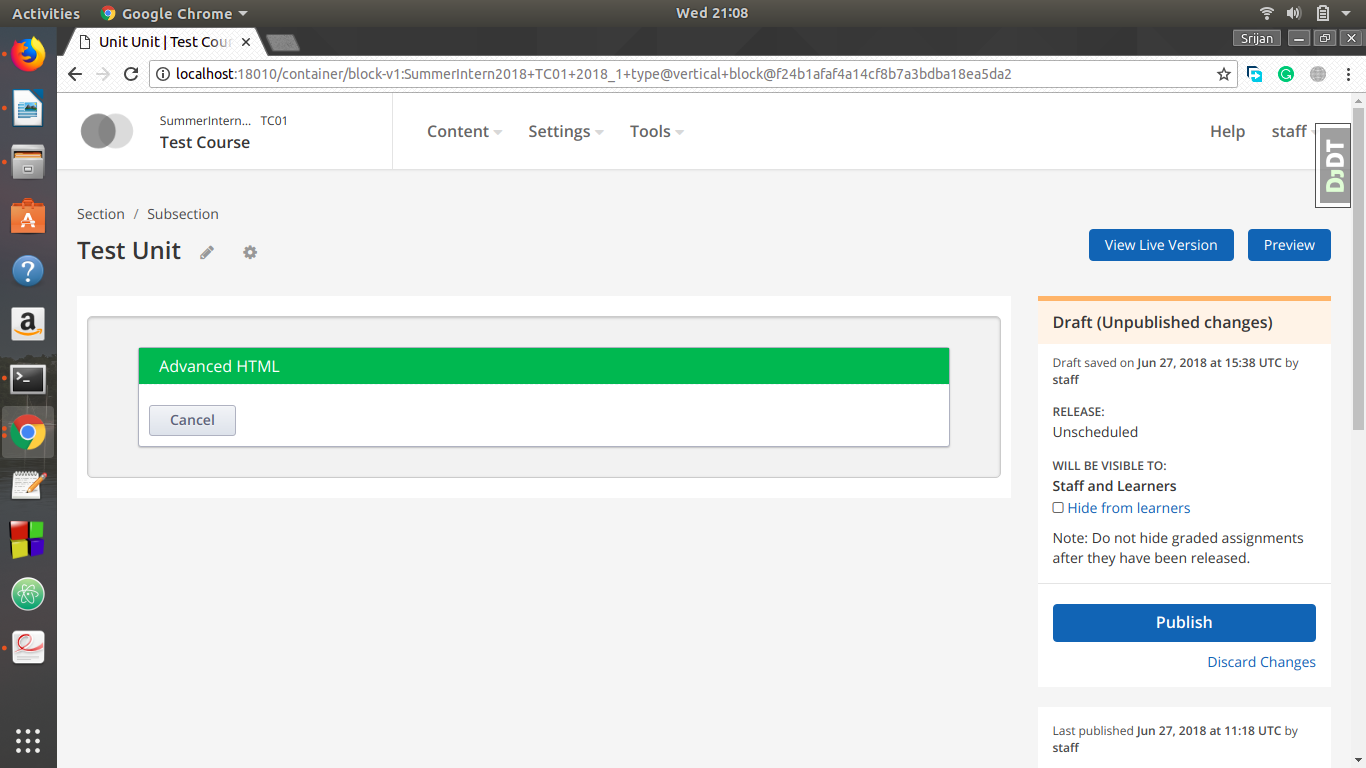
\includegraphics[width=\textwidth]{images/demo_1}
  \caption{Xblock available in advanced components}

  \vspace*{\floatsep}

  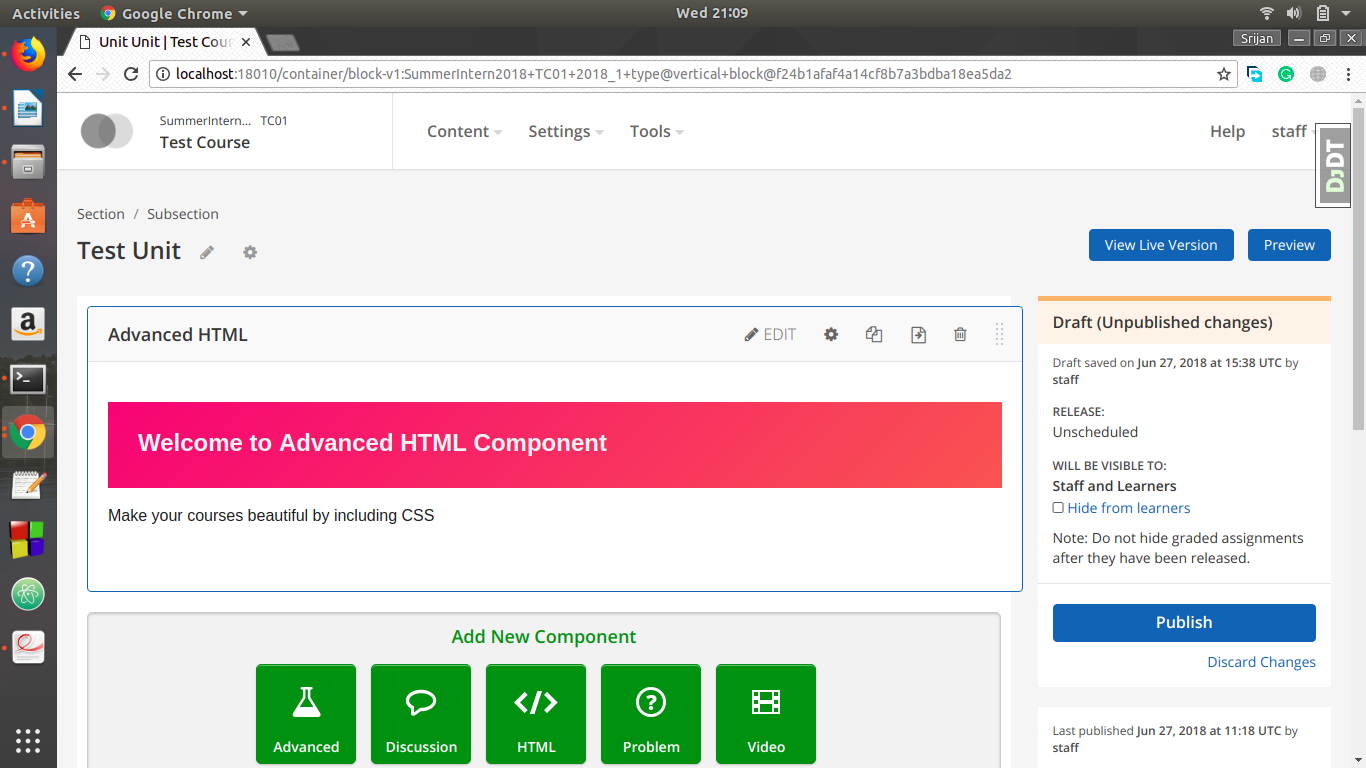
\includegraphics[width=\textwidth]{images/demo_2}
  \caption{Default content of xblock}
\end{figure}


\begin{figure}[ht]
  \centering
  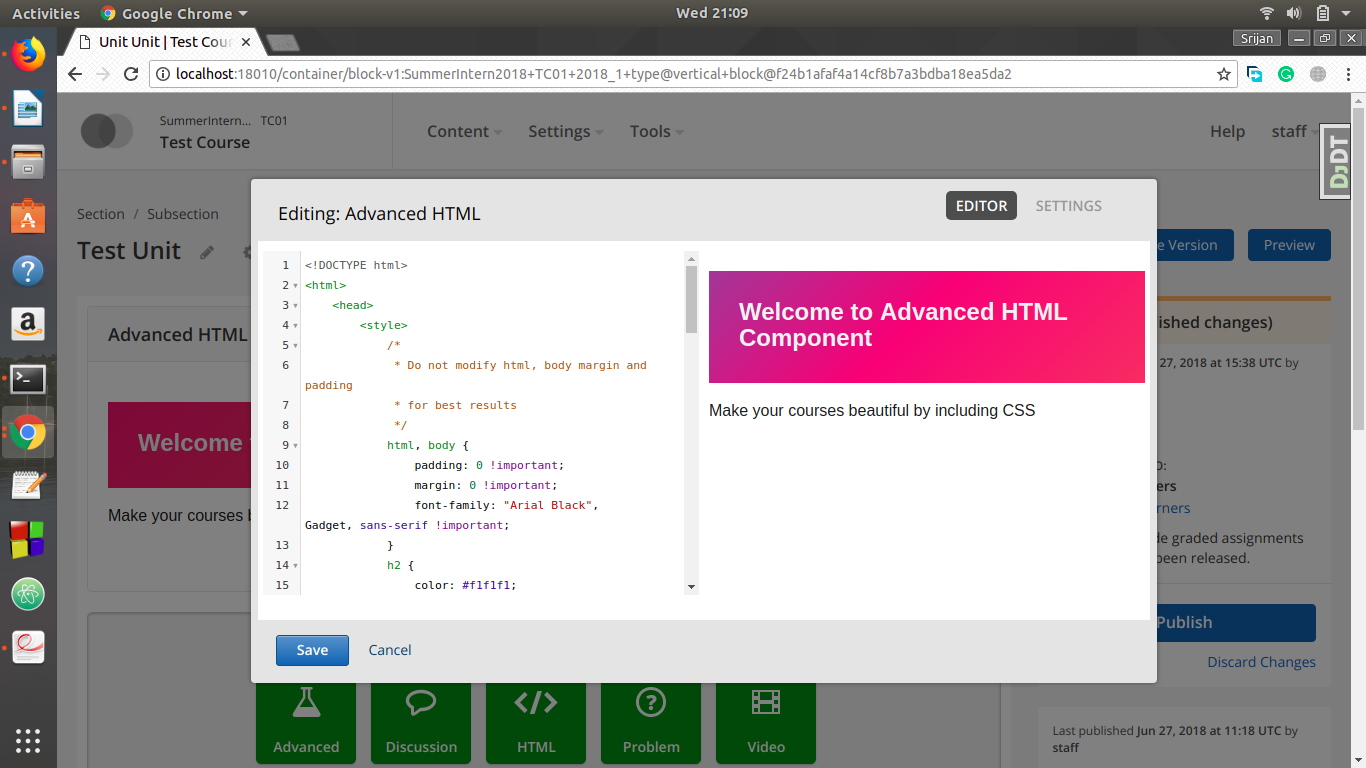
\includegraphics[width=\textwidth]{images/demo_3}
  \caption{Editor with live preview}

  \vspace*{\floatsep}

  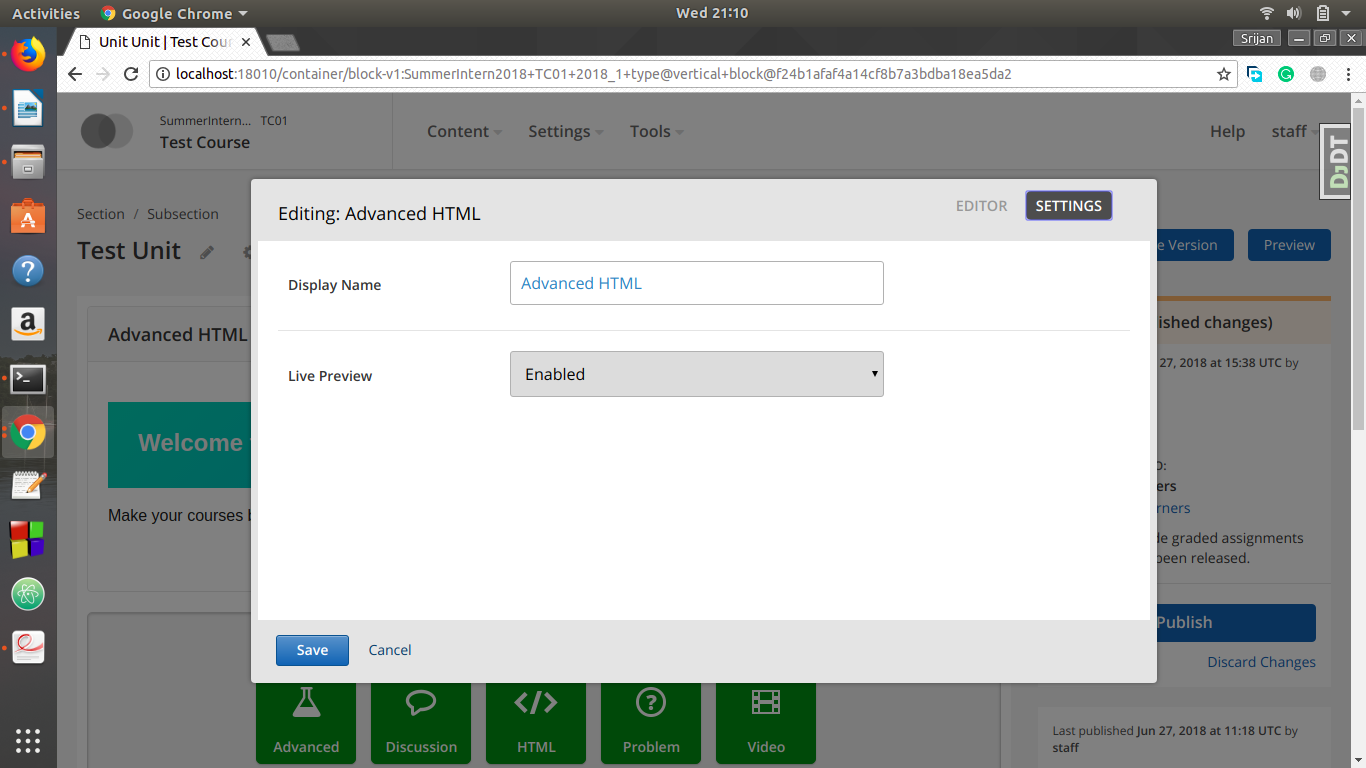
\includegraphics[width=\textwidth]{images/demo_4}
  \caption{Settings tab}
\end{figure}


\begin{figure}[ht]
  \centering
  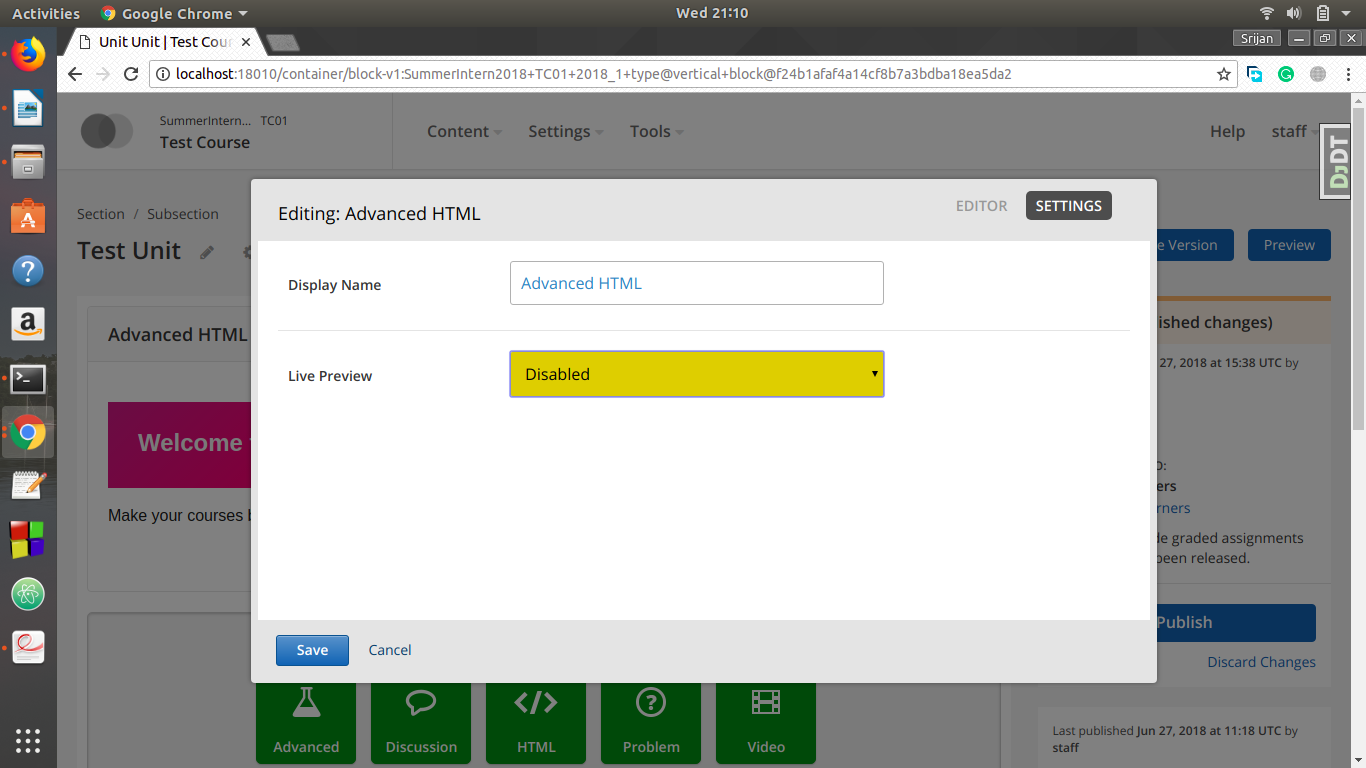
\includegraphics[width=\textwidth]{images/demo_5}
  \caption{Disabling live preview}

  \vspace*{\floatsep}

  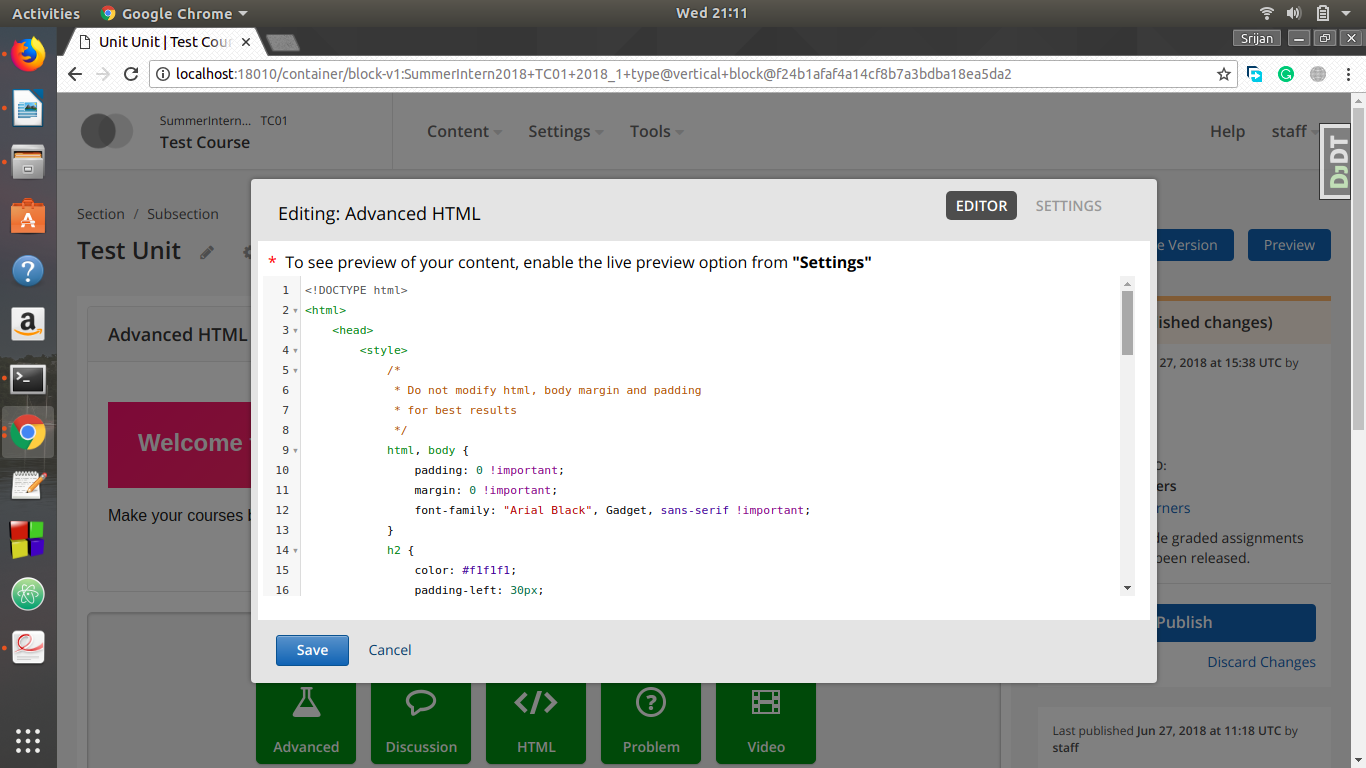
\includegraphics[width=\textwidth]{images/demo_6}
  \caption{Full width editor available}
\end{figure}

\begin{figure}[ht]
  \centering
  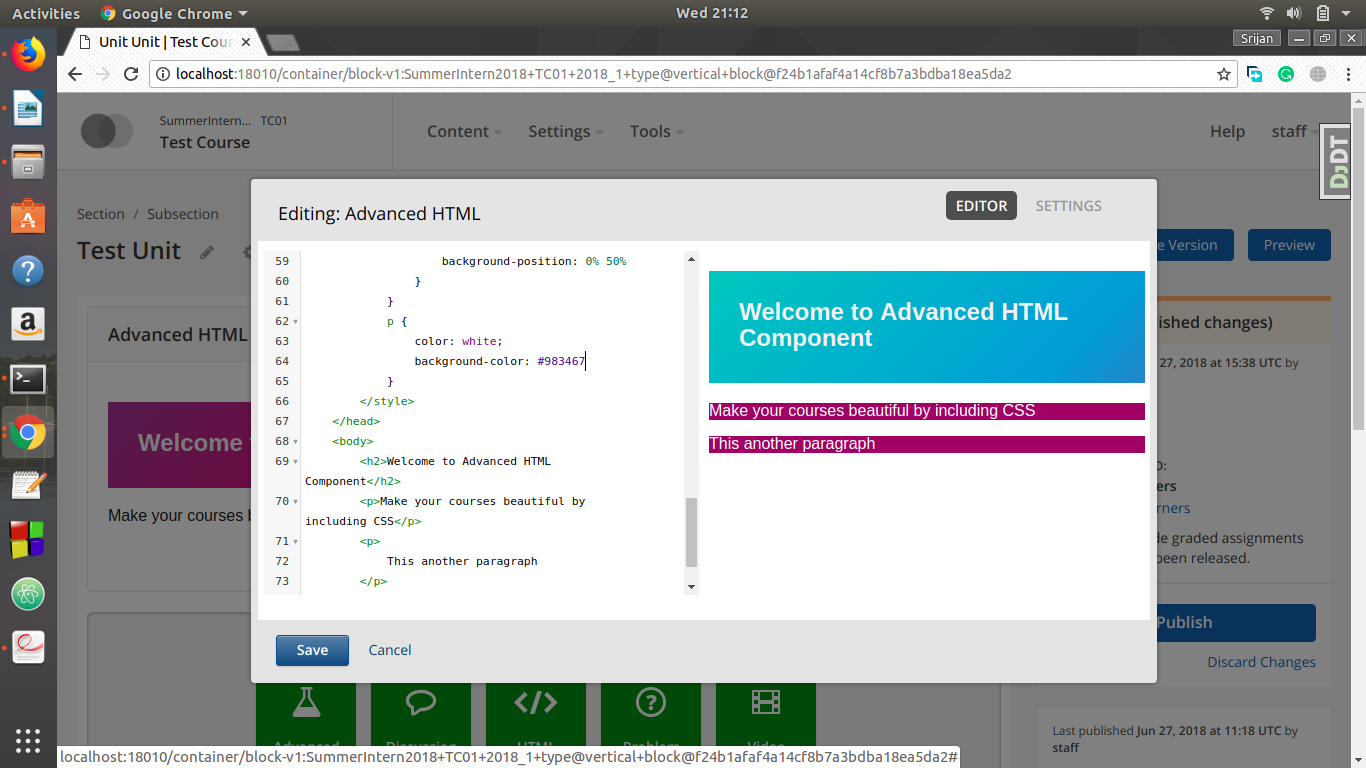
\includegraphics[width=\textwidth]{images/demo_7}
  \caption{Live preview in action}

  \vspace*{\floatsep}

  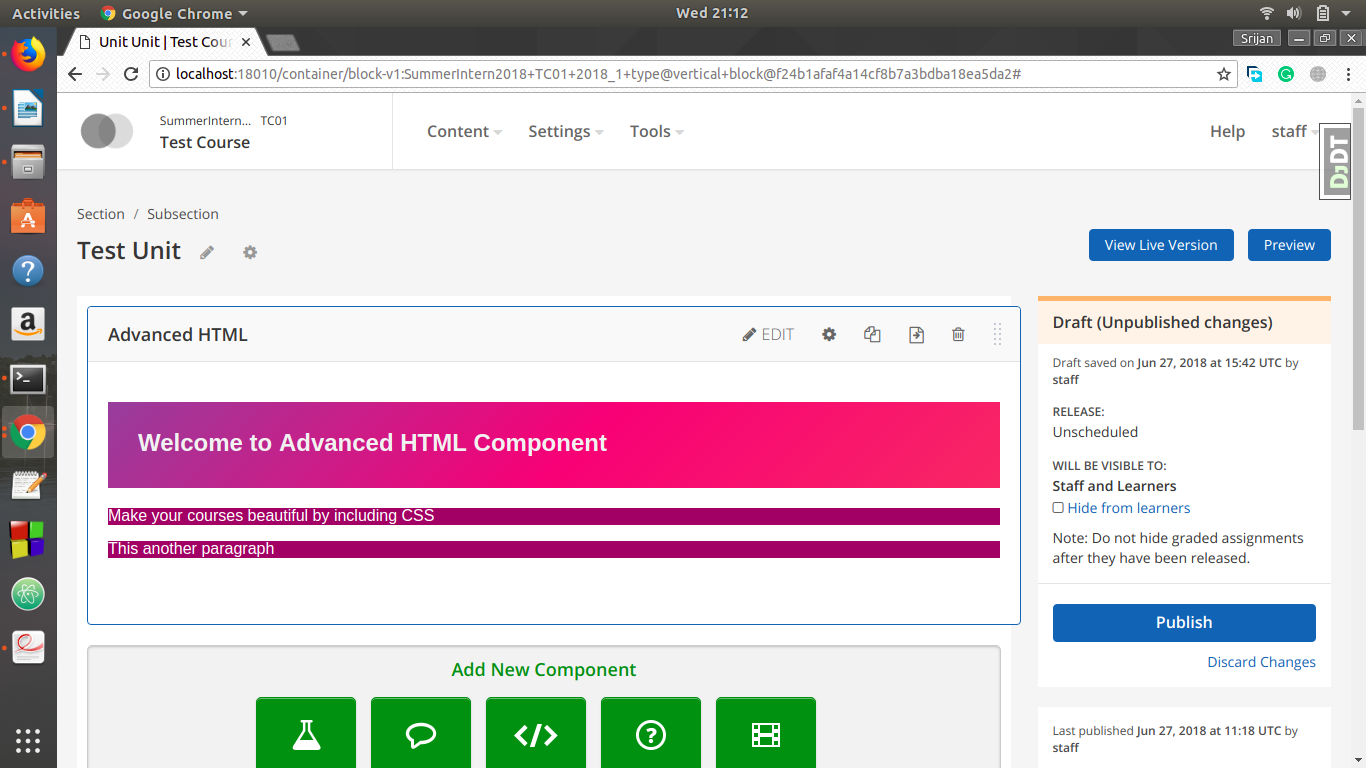
\includegraphics[width=\textwidth]{images/demo_8}
  \caption{Final component after editing content}
\end{figure}






\end{document}